\documentclass[twoside]{book}

% Packages required by doxygen
\usepackage{fixltx2e}
\usepackage{calc}
\usepackage{doxygen}
\usepackage[export]{adjustbox} % also loads graphicx
\usepackage{graphicx}
\usepackage[utf8]{inputenc}
\usepackage{makeidx}
\usepackage{multicol}
\usepackage{multirow}
\PassOptionsToPackage{warn}{textcomp}
\usepackage{textcomp}
\usepackage[nointegrals]{wasysym}
\usepackage[table]{xcolor}

% Font selection
\usepackage[T1]{fontenc}
\usepackage[scaled=.90]{helvet}
\usepackage{courier}
\usepackage{amssymb}
\usepackage{sectsty}
\renewcommand{\familydefault}{\sfdefault}
\allsectionsfont{%
  \fontseries{bc}\selectfont%
  \color{darkgray}%
}
\renewcommand{\DoxyLabelFont}{%
  \fontseries{bc}\selectfont%
  \color{darkgray}%
}
\newcommand{\+}{\discretionary{\mbox{\scriptsize$\hookleftarrow$}}{}{}}

% Page & text layout
\usepackage{geometry}
\geometry{%
  a4paper,%
  top=2.5cm,%
  bottom=2.5cm,%
  left=2.5cm,%
  right=2.5cm%
}
\tolerance=750
\hfuzz=15pt
\hbadness=750
\setlength{\emergencystretch}{15pt}
\setlength{\parindent}{0cm}
\setlength{\parskip}{3ex plus 2ex minus 2ex}
\makeatletter
\renewcommand{\paragraph}{%
  \@startsection{paragraph}{4}{0ex}{-1.0ex}{1.0ex}{%
    \normalfont\normalsize\bfseries\SS@parafont%
  }%
}
\renewcommand{\subparagraph}{%
  \@startsection{subparagraph}{5}{0ex}{-1.0ex}{1.0ex}{%
    \normalfont\normalsize\bfseries\SS@subparafont%
  }%
}
\makeatother

% Headers & footers
\usepackage{fancyhdr}
\pagestyle{fancyplain}
\fancyhead[LE]{\fancyplain{}{\bfseries\thepage}}
\fancyhead[CE]{\fancyplain{}{}}
\fancyhead[RE]{\fancyplain{}{\bfseries\leftmark}}
\fancyhead[LO]{\fancyplain{}{\bfseries\rightmark}}
\fancyhead[CO]{\fancyplain{}{}}
\fancyhead[RO]{\fancyplain{}{\bfseries\thepage}}
\fancyfoot[LE]{\fancyplain{}{}}
\fancyfoot[CE]{\fancyplain{}{}}
\fancyfoot[RE]{\fancyplain{}{\bfseries\scriptsize Generated by Doxygen }}
\fancyfoot[LO]{\fancyplain{}{\bfseries\scriptsize Generated by Doxygen }}
\fancyfoot[CO]{\fancyplain{}{}}
\fancyfoot[RO]{\fancyplain{}{}}
\renewcommand{\footrulewidth}{0.4pt}
\renewcommand{\chaptermark}[1]{%
  \markboth{#1}{}%
}
\renewcommand{\sectionmark}[1]{%
  \markright{\thesection\ #1}%
}

% Indices & bibliography
\usepackage{natbib}
\usepackage[titles]{tocloft}
\setcounter{tocdepth}{3}
\setcounter{secnumdepth}{5}
\makeindex

% Hyperlinks (required, but should be loaded last)
\usepackage{ifpdf}
\ifpdf
  \usepackage[pdftex,pagebackref=true]{hyperref}
\else
  \usepackage[ps2pdf,pagebackref=true]{hyperref}
\fi
\hypersetup{%
  colorlinks=true,%
  linkcolor=blue,%
  citecolor=blue,%
  unicode%
}

% Custom commands
\newcommand{\clearemptydoublepage}{%
  \newpage{\pagestyle{empty}\cleardoublepage}%
}

\usepackage{caption}
\captionsetup{labelsep=space,justification=centering,font={bf},singlelinecheck=off,skip=4pt,position=top}

%===== C O N T E N T S =====

\begin{document}

% Titlepage & ToC
\hypersetup{pageanchor=false,
             bookmarksnumbered=true,
             pdfencoding=unicode
            }
\pagenumbering{alph}
\begin{titlepage}
\vspace*{7cm}
\begin{center}%
{\Large Multiplayer Game }\\
\vspace*{1cm}
{\large Generated by Doxygen 1.8.13}\\
\end{center}
\end{titlepage}
\clearemptydoublepage
\pagenumbering{roman}
\tableofcontents
\clearemptydoublepage
\pagenumbering{arabic}
\hypersetup{pageanchor=true}

%--- Begin generated contents ---
\chapter{Hierarchical Index}
\section{Class Hierarchy}
This inheritance list is sorted roughly, but not completely, alphabetically\+:\begin{DoxyCompactList}
\item b2\+Contact\+Listener\begin{DoxyCompactList}
\item \contentsline{section}{Collision\+Call\+Back}{\pageref{class_collision_call_back}}{}
\end{DoxyCompactList}
\item \contentsline{section}{Coin\+Info}{\pageref{struct_coin_info}}{}
\item \contentsline{section}{Game\+Manager}{\pageref{class_game_manager}}{}
\item \contentsline{section}{Net\+Work\+Manager}{\pageref{class_net_work_manager}}{}
\item \contentsline{section}{Object}{\pageref{class_object}}{}
\begin{DoxyCompactList}
\item \contentsline{section}{Coin}{\pageref{class_coin}}{}
\item \contentsline{section}{Ground}{\pageref{class_ground}}{}
\item \contentsline{section}{Net\+Player}{\pageref{class_net_player}}{}
\item \contentsline{section}{Platform}{\pageref{class_platform}}{}
\item \contentsline{section}{Player}{\pageref{class_player}}{}
\item \contentsline{section}{Spike\+Box}{\pageref{class_spike_box}}{}
\item \contentsline{section}{Wall}{\pageref{class_wall}}{}
\end{DoxyCompactList}
\item \contentsline{section}{Player\+Info}{\pageref{struct_player_info}}{}
\item \contentsline{section}{Points\+Pos\+Users\+Text}{\pageref{struct_points_pos_users_text}}{}
\item \contentsline{section}{Scene}{\pageref{class_scene}}{}
\item \contentsline{section}{Spike\+Box\+Info}{\pageref{struct_spike_box_info}}{}
\item \contentsline{section}{Vec2}{\pageref{struct_vec2}}{}
\end{DoxyCompactList}

\chapter{Class Index}
\section{Class List}
Here are the classes, structs, unions and interfaces with brief descriptions\+:\begin{DoxyCompactList}
\item\contentsline{section}{\hyperlink{class_coin}{Coin} }{\pageref{class_coin}}{}
\item\contentsline{section}{\hyperlink{struct_coin_info}{Coin\+Info} }{\pageref{struct_coin_info}}{}
\item\contentsline{section}{\hyperlink{class_collision_call_back}{Collision\+Call\+Back} }{\pageref{class_collision_call_back}}{}
\item\contentsline{section}{\hyperlink{class_game_manager}{Game\+Manager} }{\pageref{class_game_manager}}{}
\item\contentsline{section}{\hyperlink{class_ground}{Ground} }{\pageref{class_ground}}{}
\item\contentsline{section}{\hyperlink{class_net_player}{Net\+Player} }{\pageref{class_net_player}}{}
\item\contentsline{section}{\hyperlink{class_net_work_manager}{Net\+Work\+Manager} }{\pageref{class_net_work_manager}}{}
\item\contentsline{section}{\hyperlink{class_object}{Object} }{\pageref{class_object}}{}
\item\contentsline{section}{\hyperlink{class_platform}{Platform} }{\pageref{class_platform}}{}
\item\contentsline{section}{\hyperlink{class_player}{Player} }{\pageref{class_player}}{}
\item\contentsline{section}{\hyperlink{struct_player_info}{Player\+Info} }{\pageref{struct_player_info}}{}
\item\contentsline{section}{\hyperlink{struct_points_pos_users_text}{Points\+Pos\+Users\+Text} }{\pageref{struct_points_pos_users_text}}{}
\item\contentsline{section}{\hyperlink{class_scene}{Scene} }{\pageref{class_scene}}{}
\item\contentsline{section}{\hyperlink{class_spike_box}{Spike\+Box} }{\pageref{class_spike_box}}{}
\item\contentsline{section}{\hyperlink{struct_spike_box_info}{Spike\+Box\+Info} }{\pageref{struct_spike_box_info}}{}
\item\contentsline{section}{\hyperlink{struct_vec2}{Vec2} }{\pageref{struct_vec2}}{}
\item\contentsline{section}{\hyperlink{class_wall}{Wall} }{\pageref{class_wall}}{}
\end{DoxyCompactList}

\chapter{Class Documentation}
\hypertarget{class_coin}{}\section{Coin Class Reference}
\label{class_coin}\index{Coin@{Coin}}
Inheritance diagram for Coin\+:\begin{figure}[H]
\begin{center}
\leavevmode
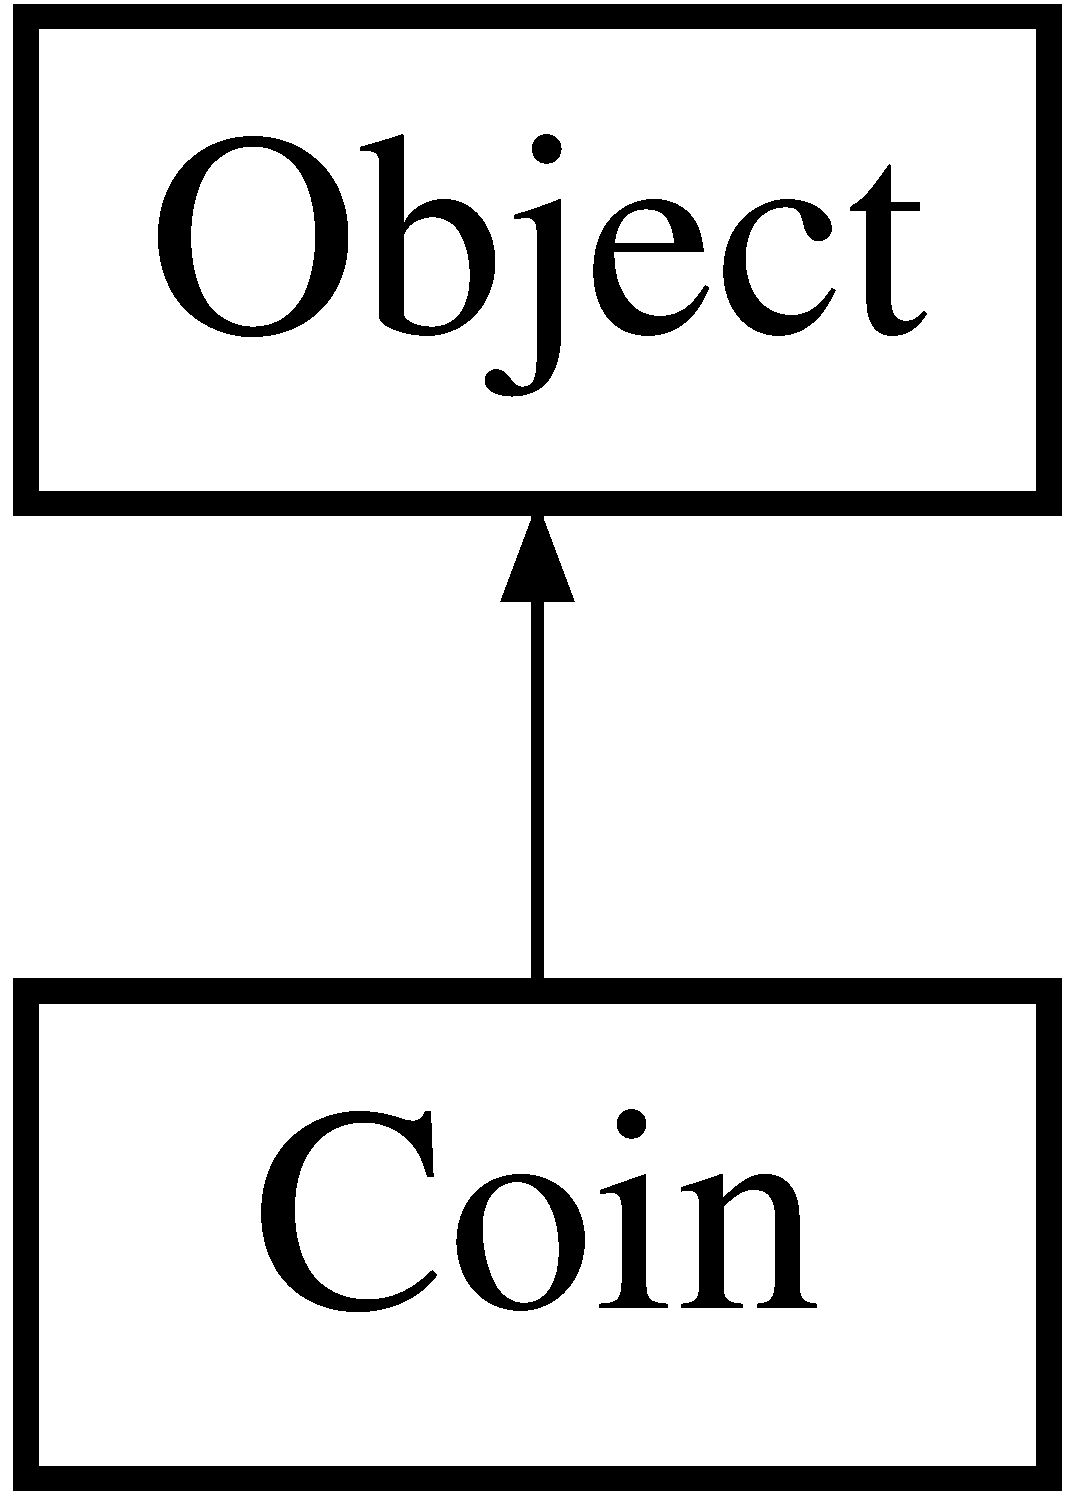
\includegraphics[height=2.000000cm]{class_coin}
\end{center}
\end{figure}
\subsection*{Public Member Functions}
\begin{DoxyCompactItemize}
\item 
\mbox{\Hypertarget{class_coin_ad0371a6d98c194a0f6de615206829b16}\label{class_coin_ad0371a6d98c194a0f6de615206829b16}} 
\hyperlink{class_coin_ad0371a6d98c194a0f6de615206829b16}{$\sim$\+Coin} ()
\begin{DoxyCompactList}\small\item\em Destructor. \end{DoxyCompactList}\item 
\mbox{\Hypertarget{class_coin_ace98dea331520b1bdd75213da9765b63}\label{class_coin_ace98dea331520b1bdd75213da9765b63}} 
\hyperlink{class_coin_ace98dea331520b1bdd75213da9765b63}{Coin} (\hyperlink{struct_vec2}{Vec2} position, \hyperlink{struct_vec2}{Vec2} scale, Body\+Type type, float32 density, float32 friction, char $\ast$texture, \hyperlink{struct_vec2}{Vec2} sprite\+Origin)
\begin{DoxyCompactList}\small\item\em Constructor. \end{DoxyCompactList}\item 
\mbox{\Hypertarget{class_coin_abe676fdd24be69f9b605a59076d5a90d}\label{class_coin_abe676fdd24be69f9b605a59076d5a90d}} 
virtual void \hyperlink{class_coin_abe676fdd24be69f9b605a59076d5a90d}{Init} () override
\begin{DoxyCompactList}\small\item\em Init. \end{DoxyCompactList}\item 
\mbox{\Hypertarget{class_coin_a13e1d3025965f73a63e34e9c6a21d8e0}\label{class_coin_a13e1d3025965f73a63e34e9c6a21d8e0}} 
virtual void \hyperlink{class_coin_a13e1d3025965f73a63e34e9c6a21d8e0}{Input} () override
\begin{DoxyCompactList}\small\item\em Input. \end{DoxyCompactList}\item 
\mbox{\Hypertarget{class_coin_a3638832a26fc17f40d04e8e590cf9963}\label{class_coin_a3638832a26fc17f40d04e8e590cf9963}} 
virtual void \hyperlink{class_coin_a3638832a26fc17f40d04e8e590cf9963}{Update} () override
\begin{DoxyCompactList}\small\item\em Update. \end{DoxyCompactList}\item 
\mbox{\Hypertarget{class_coin_a4fbc44581a02121f6c4e6b93b493175d}\label{class_coin_a4fbc44581a02121f6c4e6b93b493175d}} 
virtual void \hyperlink{class_coin_a4fbc44581a02121f6c4e6b93b493175d}{Reset} () override
\begin{DoxyCompactList}\small\item\em Reset. \end{DoxyCompactList}\item 
virtual void \hyperlink{class_coin_aa6b47cadab21693854c2c4f8266a5ac1}{Collision} (\hyperlink{class_object}{Object} $\ast$instigator) override
\item 
\mbox{\Hypertarget{class_coin_af2b1a914f49d5fcaf5b2c1ce74d5b065}\label{class_coin_af2b1a914f49d5fcaf5b2c1ce74d5b065}} 
virtual Define\+Type \hyperlink{class_coin_af2b1a914f49d5fcaf5b2c1ce74d5b065}{get\+Define\+Type} () override
\begin{DoxyCompactList}\small\item\em Type of object. \end{DoxyCompactList}\item 
\mbox{\Hypertarget{class_coin_a599acd6db3cba922df144bad324a1b19}\label{class_coin_a599acd6db3cba922df144bad324a1b19}} 
void \hyperlink{class_coin_a599acd6db3cba922df144bad324a1b19}{Move} ()
\begin{DoxyCompactList}\small\item\em Move. \end{DoxyCompactList}\end{DoxyCompactItemize}
\subsection*{Private Attributes}
\begin{DoxyCompactItemize}
\item 
\mbox{\Hypertarget{class_coin_a4a5f701e25d7c98577af66a3de491946}\label{class_coin_a4a5f701e25d7c98577af66a3de491946}} 
bool \hyperlink{class_coin_a4a5f701e25d7c98577af66a3de491946}{Is\+Capture}
\begin{DoxyCompactList}\small\item\em Control if somebody capture the coin. \end{DoxyCompactList}\item 
\mbox{\Hypertarget{class_coin_a7ab98ec00c278f1e4adb0e0988b10cf2}\label{class_coin_a7ab98ec00c278f1e4adb0e0988b10cf2}} 
int \hyperlink{class_coin_a7ab98ec00c278f1e4adb0e0988b10cf2}{Where\+To\+Move}
\begin{DoxyCompactList}\small\item\em Random for next position. \end{DoxyCompactList}\end{DoxyCompactItemize}
\subsection*{Additional Inherited Members}


\subsection{Member Function Documentation}
\mbox{\Hypertarget{class_coin_aa6b47cadab21693854c2c4f8266a5ac1}\label{class_coin_aa6b47cadab21693854c2c4f8266a5ac1}} 
\index{Coin@{Coin}!Collision@{Collision}}
\index{Collision@{Collision}!Coin@{Coin}}
\subsubsection{\texorpdfstring{Collision()}{Collision()}}
{\footnotesize\ttfamily virtual void Coin\+::\+Collision (\begin{DoxyParamCaption}\item[{\hyperlink{class_object}{Object} $\ast$}]{instigator }\end{DoxyParamCaption})\hspace{0.3cm}{\ttfamily [override]}, {\ttfamily [virtual]}}

Collision with other objects 
\begin{DoxyParams}{Parameters}
{\em instigator} & Objects name to collide with. \\
\hline
\end{DoxyParams}


Reimplemented from \hyperlink{class_object_a0af60ea226dcb885e69483452d34a47a}{Object}.



The documentation for this class was generated from the following file\+:\begin{DoxyCompactItemize}
\item 
D\+:/\+Multiplayer/include/coin.\+h\end{DoxyCompactItemize}

\hypertarget{struct_coin_info}{}\section{Coin\+Info Struct Reference}
\label{struct_coin_info}\index{Coin\+Info@{Coin\+Info}}


{\ttfamily \#include $<$networkmanager.\+h$>$}

\subsection*{Public Attributes}
\begin{DoxyCompactItemize}
\item 
\mbox{\Hypertarget{struct_coin_info_abd8a234b9f1b4357dfbb2fdfc9b101c0}\label{struct_coin_info_abd8a234b9f1b4357dfbb2fdfc9b101c0}} 
float {\bfseries PosX}
\item 
\mbox{\Hypertarget{struct_coin_info_ae14323c2d25b8560db89f05475618697}\label{struct_coin_info_ae14323c2d25b8560db89f05475618697}} 
float {\bfseries PosY}
\item 
\mbox{\Hypertarget{struct_coin_info_a52aa89d376182bb0d2f44d2eac17b86f}\label{struct_coin_info_a52aa89d376182bb0d2f44d2eac17b86f}} 
float {\bfseries Rotation}
\end{DoxyCompactItemize}


\subsection{Detailed Description}
Struct All the information that the coin needs to receive and send 

The documentation for this struct was generated from the following file\+:\begin{DoxyCompactItemize}
\item 
D\+:/\+Multiplayer/include/networkmanager.\+h\end{DoxyCompactItemize}

\hypertarget{class_collision_call_back}{}\section{Collision\+Call\+Back Class Reference}
\label{class_collision_call_back}\index{Collision\+Call\+Back@{Collision\+Call\+Back}}
Inheritance diagram for Collision\+Call\+Back\+:\begin{figure}[H]
\begin{center}
\leavevmode
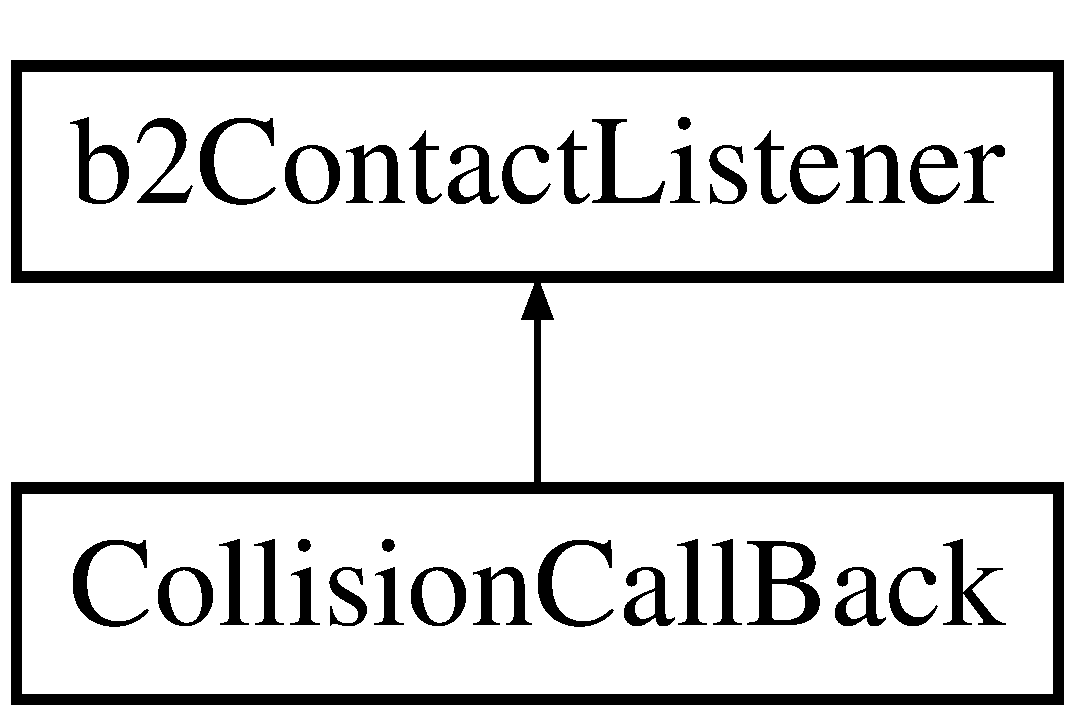
\includegraphics[height=2.000000cm]{class_collision_call_back}
\end{center}
\end{figure}
\subsection*{Public Member Functions}
\begin{DoxyCompactItemize}
\item 
\mbox{\Hypertarget{class_collision_call_back_a942cfb9f0d9eb682e56ee9f298d5b3b0}\label{class_collision_call_back_a942cfb9f0d9eb682e56ee9f298d5b3b0}} 
virtual void \hyperlink{class_collision_call_back_a942cfb9f0d9eb682e56ee9f298d5b3b0}{Begin\+Contact} (b2\+Contact $\ast$contact) override
\begin{DoxyCompactList}\small\item\em Box2D collision start listener. \end{DoxyCompactList}\item 
\mbox{\Hypertarget{class_collision_call_back_af8c0e7c724569fa711a03f1ba1906c0f}\label{class_collision_call_back_af8c0e7c724569fa711a03f1ba1906c0f}} 
virtual void \hyperlink{class_collision_call_back_af8c0e7c724569fa711a03f1ba1906c0f}{End\+Contact} (b2\+Contact $\ast$contact) override
\begin{DoxyCompactList}\small\item\em Box2D collision end listener. \end{DoxyCompactList}\end{DoxyCompactItemize}


The documentation for this class was generated from the following file\+:\begin{DoxyCompactItemize}
\item 
D\+:/\+Multiplayer/include/collisioncallback.\+h\end{DoxyCompactItemize}

\hypertarget{class_game_manager}{}\section{Game\+Manager Class Reference}
\label{class_game_manager}\index{Game\+Manager@{Game\+Manager}}
\subsection*{Public Member Functions}
\begin{DoxyCompactItemize}
\item 
\mbox{\Hypertarget{class_game_manager_a41d7c3afcf14f85e3716210e06b2ef20}\label{class_game_manager_a41d7c3afcf14f85e3716210e06b2ef20}} 
b2\+World $\ast$ \hyperlink{class_game_manager_a41d7c3afcf14f85e3716210e06b2ef20}{Get\+World} ()
\begin{DoxyCompactList}\small\item\em Get World. \end{DoxyCompactList}\item 
\mbox{\Hypertarget{class_game_manager_a27a899cc5544c30719e8b57ae93d7ffc}\label{class_game_manager_a27a899cc5544c30719e8b57ae93d7ffc}} 
sf\+::\+Render\+Window $\ast$ \hyperlink{class_game_manager_a27a899cc5544c30719e8b57ae93d7ffc}{Get\+Window} ()
\begin{DoxyCompactList}\small\item\em Get Window. \end{DoxyCompactList}\item 
\mbox{\Hypertarget{class_game_manager_ac227cf3926f59e4c2bf6420bfd1a90e6}\label{class_game_manager_ac227cf3926f59e4c2bf6420bfd1a90e6}} 
void \hyperlink{class_game_manager_ac227cf3926f59e4c2bf6420bfd1a90e6}{Get\+Input} ()
\begin{DoxyCompactList}\small\item\em Get Input. \end{DoxyCompactList}\item 
\mbox{\Hypertarget{class_game_manager_ad27dc1c25f99244acafa5832bc2424a4}\label{class_game_manager_ad27dc1c25f99244acafa5832bc2424a4}} 
void \hyperlink{class_game_manager_ad27dc1c25f99244acafa5832bc2424a4}{Init} ()
\begin{DoxyCompactList}\small\item\em Init. \end{DoxyCompactList}\item 
\mbox{\Hypertarget{class_game_manager_a3aa49c2431d703ba1a5aa9183589e593}\label{class_game_manager_a3aa49c2431d703ba1a5aa9183589e593}} 
void \hyperlink{class_game_manager_a3aa49c2431d703ba1a5aa9183589e593}{Input} ()
\begin{DoxyCompactList}\small\item\em Input. \end{DoxyCompactList}\item 
\mbox{\Hypertarget{class_game_manager_af3bb4452ac262ec8a68dcc3eea2f0124}\label{class_game_manager_af3bb4452ac262ec8a68dcc3eea2f0124}} 
void \hyperlink{class_game_manager_af3bb4452ac262ec8a68dcc3eea2f0124}{Update} ()
\begin{DoxyCompactList}\small\item\em Update. \end{DoxyCompactList}\item 
\mbox{\Hypertarget{class_game_manager_ac1bd6de1844831d097b24a13a0e6a5a5}\label{class_game_manager_ac1bd6de1844831d097b24a13a0e6a5a5}} 
void \hyperlink{class_game_manager_ac1bd6de1844831d097b24a13a0e6a5a5}{Render} ()
\begin{DoxyCompactList}\small\item\em Render. \end{DoxyCompactList}\item 
\hyperlink{class_object}{Object} $\ast$ \hyperlink{class_game_manager_acc61ce12b7ed93580b4a585389bcc968}{Create\+Object} (\hyperlink{struct_vec2}{Vec2} position, \hyperlink{struct_vec2}{Vec2} scale, Body\+Type type, float32 density, float32 friction, char $\ast$texture, \hyperlink{struct_vec2}{Vec2} sprite\+Origin, Define\+Type Spawn\+Type)
\item 
\mbox{\Hypertarget{class_game_manager_a53219287fbbdd657a2fc34316d83665b}\label{class_game_manager_a53219287fbbdd657a2fc34316d83665b}} 
void \hyperlink{class_game_manager_a53219287fbbdd657a2fc34316d83665b}{Reset} ()
\begin{DoxyCompactList}\small\item\em Reset the game. \end{DoxyCompactList}\item 
\mbox{\Hypertarget{class_game_manager_a472b4130e5cff04138c30189d2b3f890}\label{class_game_manager_a472b4130e5cff04138c30189d2b3f890}} 
void \hyperlink{class_game_manager_a472b4130e5cff04138c30189d2b3f890}{Init\+I\+M\+G\+UI} ()
\begin{DoxyCompactList}\small\item\em Init Imgui. \end{DoxyCompactList}\item 
\mbox{\Hypertarget{class_game_manager_ae8672e78febd97d68dd42b9e843b3527}\label{class_game_manager_ae8672e78febd97d68dd42b9e843b3527}} 
void \hyperlink{class_game_manager_ae8672e78febd97d68dd42b9e843b3527}{Update\+I\+M\+G\+UI} ()
\begin{DoxyCompactList}\small\item\em Update Imgui. \end{DoxyCompactList}\item 
\mbox{\Hypertarget{class_game_manager_a2bb8e4c7d0c8438a4c2bbeb17c808c37}\label{class_game_manager_a2bb8e4c7d0c8438a4c2bbeb17c808c37}} 
void \hyperlink{class_game_manager_a2bb8e4c7d0c8438a4c2bbeb17c808c37}{Render\+I\+M\+G\+UI} ()
\begin{DoxyCompactList}\small\item\em Render Imgui. \end{DoxyCompactList}\item 
\mbox{\Hypertarget{class_game_manager_a957ca0e6277341d2473e6b9ba3c2346f}\label{class_game_manager_a957ca0e6277341d2473e6b9ba3c2346f}} 
void \hyperlink{class_game_manager_a957ca0e6277341d2473e6b9ba3c2346f}{End\+I\+M\+G\+UI} ()
\begin{DoxyCompactList}\small\item\em Render Imgui. \end{DoxyCompactList}\item 
\mbox{\Hypertarget{class_game_manager_a6b74f0e67d6407fe9852250aff423269}\label{class_game_manager_a6b74f0e67d6407fe9852250aff423269}} 
void \hyperlink{class_game_manager_a6b74f0e67d6407fe9852250aff423269}{Shut\+Down\+I\+M\+G\+UI} ()
\begin{DoxyCompactList}\small\item\em Close Imgui. \end{DoxyCompactList}\end{DoxyCompactItemize}
\subsection*{Static Public Member Functions}
\begin{DoxyCompactItemize}
\item 
\mbox{\Hypertarget{class_game_manager_ad2f647253a04cdf60e3bff6fede8a30b}\label{class_game_manager_ad2f647253a04cdf60e3bff6fede8a30b}} 
static \hyperlink{class_game_manager}{Game\+Manager} $\ast$ \hyperlink{class_game_manager_ad2f647253a04cdf60e3bff6fede8a30b}{Get\+Instance} ()
\begin{DoxyCompactList}\small\item\em Get the instance. \end{DoxyCompactList}\end{DoxyCompactItemize}
\subsection*{Public Attributes}
\begin{DoxyCompactItemize}
\item 
\mbox{\Hypertarget{class_game_manager_aff46e2ad7c2b424f25e3777aade8c87a}\label{class_game_manager_aff46e2ad7c2b424f25e3777aade8c87a}} 
sf\+::\+Clock \hyperlink{class_game_manager_aff46e2ad7c2b424f25e3777aade8c87a}{delta\+Clock}
\begin{DoxyCompactList}\small\item\em Clock. \end{DoxyCompactList}\end{DoxyCompactItemize}
\subsection*{Private Attributes}
\begin{DoxyCompactItemize}
\item 
\mbox{\Hypertarget{class_game_manager_a0216b1732c0596be052ccfee53f27e19}\label{class_game_manager_a0216b1732c0596be052ccfee53f27e19}} 
sf\+::\+Render\+Window $\ast$ \hyperlink{class_game_manager_a0216b1732c0596be052ccfee53f27e19}{Window}
\begin{DoxyCompactList}\small\item\em Window variable. \end{DoxyCompactList}\item 
\mbox{\Hypertarget{class_game_manager_ab530dfeb913a8a4682e69dab57b2eff0}\label{class_game_manager_ab530dfeb913a8a4682e69dab57b2eff0}} 
b2\+World $\ast$ \hyperlink{class_game_manager_ab530dfeb913a8a4682e69dab57b2eff0}{World}
\begin{DoxyCompactList}\small\item\em World variable. \end{DoxyCompactList}\item 
\mbox{\Hypertarget{class_game_manager_a3b42dce4375c2259786fc6a4c4ace2ea}\label{class_game_manager_a3b42dce4375c2259786fc6a4c4ace2ea}} 
std\+::vector$<$ \hyperlink{class_object}{Object} $\ast$ $>$ \hyperlink{class_game_manager_a3b42dce4375c2259786fc6a4c4ace2ea}{Objects}
\begin{DoxyCompactList}\small\item\em Contains all the objects created. \end{DoxyCompactList}\end{DoxyCompactItemize}
\subsection*{Static Private Attributes}
\begin{DoxyCompactItemize}
\item 
\mbox{\Hypertarget{class_game_manager_a8f823a490b0110b09be5bd8badbf792a}\label{class_game_manager_a8f823a490b0110b09be5bd8badbf792a}} 
static \hyperlink{class_game_manager}{Game\+Manager} $\ast$ \hyperlink{class_game_manager_a8f823a490b0110b09be5bd8badbf792a}{Instance}
\begin{DoxyCompactList}\small\item\em Instance variable. \end{DoxyCompactList}\end{DoxyCompactItemize}


\subsection{Member Function Documentation}
\mbox{\Hypertarget{class_game_manager_acc61ce12b7ed93580b4a585389bcc968}\label{class_game_manager_acc61ce12b7ed93580b4a585389bcc968}} 
\index{Game\+Manager@{Game\+Manager}!Create\+Object@{Create\+Object}}
\index{Create\+Object@{Create\+Object}!Game\+Manager@{Game\+Manager}}
\subsubsection{\texorpdfstring{Create\+Object()}{CreateObject()}}
{\footnotesize\ttfamily \hyperlink{class_object}{Object}$\ast$ Game\+Manager\+::\+Create\+Object (\begin{DoxyParamCaption}\item[{\hyperlink{struct_vec2}{Vec2}}]{position,  }\item[{\hyperlink{struct_vec2}{Vec2}}]{scale,  }\item[{Body\+Type}]{type,  }\item[{float32}]{density,  }\item[{float32}]{friction,  }\item[{char $\ast$}]{texture,  }\item[{\hyperlink{struct_vec2}{Vec2}}]{sprite\+Origin,  }\item[{Define\+Type}]{Spawn\+Type }\end{DoxyParamCaption})}

Creates an object 
\begin{DoxyParams}{Parameters}
{\em position} & Position x and y. \\
\hline
{\em scale} & Width and height. \\
\hline
{\em type} & Static or dinamic object. \\
\hline
{\em density} & Density of the object. \\
\hline
{\em friction} & Friction of the object. \\
\hline
{\em texture} & Name of the image. \\
\hline
{\em sprite\+Origin} & Width/2 and height/2. \\
\hline
{\em Spawn\+Type} & Type of object. \\
\hline
\end{DoxyParams}
\begin{DoxyReturn}{Returns}
An object 
\end{DoxyReturn}


The documentation for this class was generated from the following file\+:\begin{DoxyCompactItemize}
\item 
D\+:/\+Multiplayer/include/gamemanager.\+h\end{DoxyCompactItemize}

\hypertarget{class_ground}{}\section{Ground Class Reference}
\label{class_ground}\index{Ground@{Ground}}
Inheritance diagram for Ground\+:\begin{figure}[H]
\begin{center}
\leavevmode
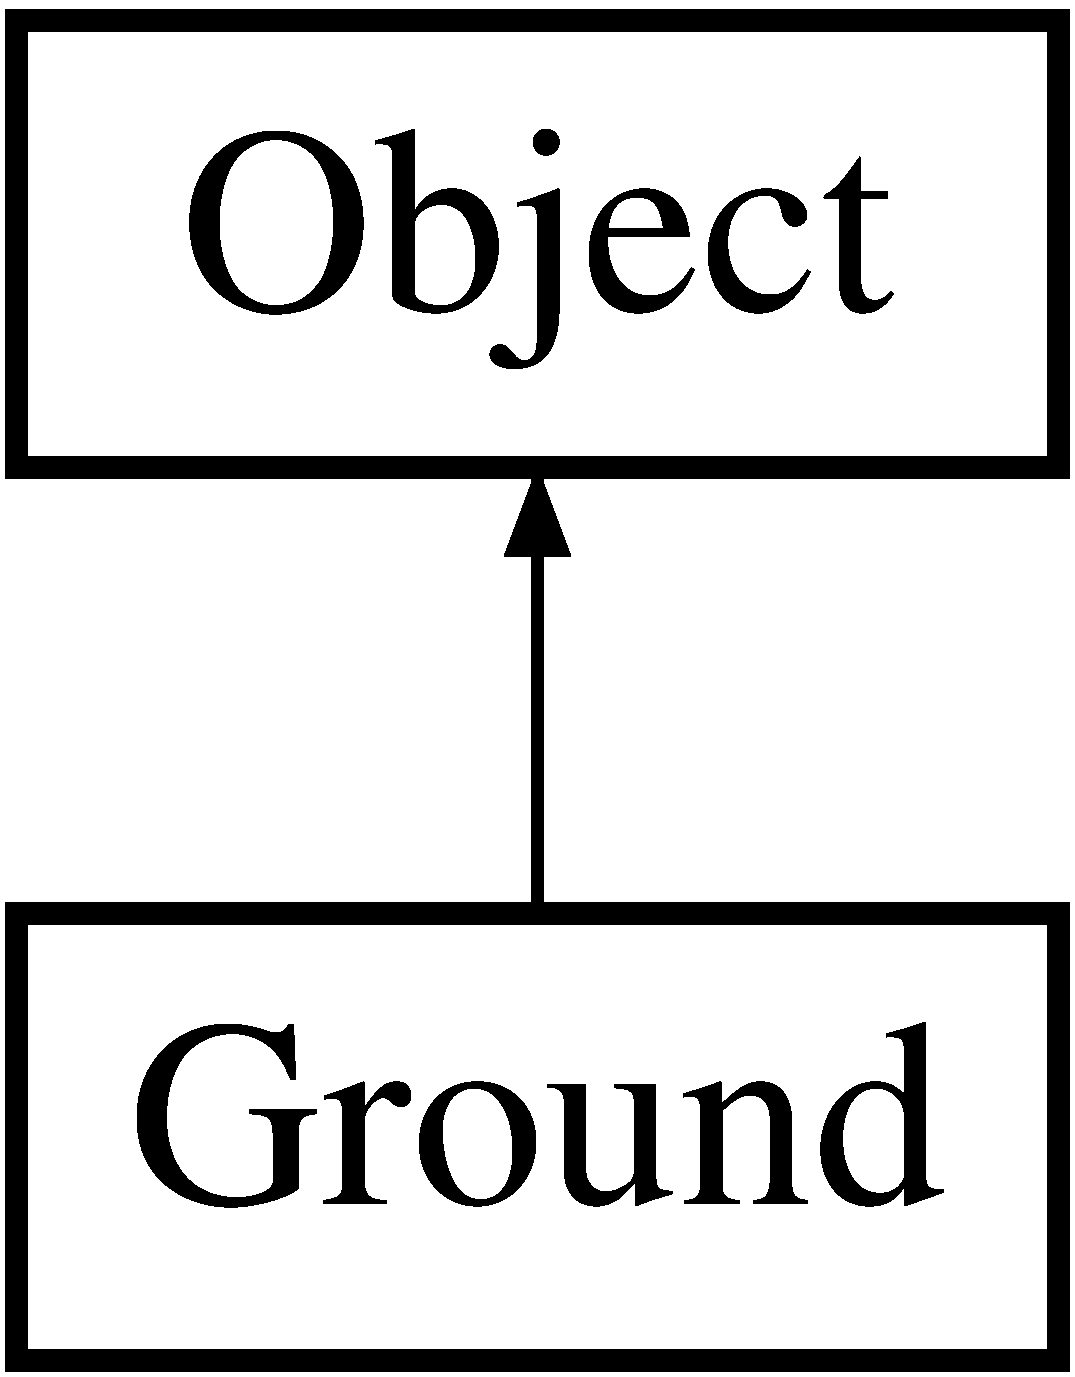
\includegraphics[height=2.000000cm]{class_ground}
\end{center}
\end{figure}
\subsection*{Public Member Functions}
\begin{DoxyCompactItemize}
\item 
\mbox{\Hypertarget{class_ground_ad39c80052f8357c29b364384c3488e4e}\label{class_ground_ad39c80052f8357c29b364384c3488e4e}} 
\hyperlink{class_ground_ad39c80052f8357c29b364384c3488e4e}{$\sim$\+Ground} ()
\begin{DoxyCompactList}\small\item\em Destructor. \end{DoxyCompactList}\item 
\mbox{\Hypertarget{class_ground_a8710ce641b9a630ebae69637159e2354}\label{class_ground_a8710ce641b9a630ebae69637159e2354}} 
\hyperlink{class_ground_a8710ce641b9a630ebae69637159e2354}{Ground} (\hyperlink{struct_vec2}{Vec2} position, \hyperlink{struct_vec2}{Vec2} scale, Body\+Type type, float32 density, float32 friction, char $\ast$texture, \hyperlink{struct_vec2}{Vec2} sprite\+Origin)
\begin{DoxyCompactList}\small\item\em Constructor. \end{DoxyCompactList}\item 
\mbox{\Hypertarget{class_ground_af3203f3fd7dce00c7c69736e46d555c1}\label{class_ground_af3203f3fd7dce00c7c69736e46d555c1}} 
virtual void \hyperlink{class_ground_af3203f3fd7dce00c7c69736e46d555c1}{Init} () override
\begin{DoxyCompactList}\small\item\em Init. \end{DoxyCompactList}\item 
\mbox{\Hypertarget{class_ground_a862cf7a6d242ab2380125c24c86b3776}\label{class_ground_a862cf7a6d242ab2380125c24c86b3776}} 
virtual void \hyperlink{class_ground_a862cf7a6d242ab2380125c24c86b3776}{Input} () override
\begin{DoxyCompactList}\small\item\em Input. \end{DoxyCompactList}\item 
\mbox{\Hypertarget{class_ground_a75d1be9fc439e7f8cb6193abfcef2da5}\label{class_ground_a75d1be9fc439e7f8cb6193abfcef2da5}} 
virtual void \hyperlink{class_ground_a75d1be9fc439e7f8cb6193abfcef2da5}{Update} () override
\begin{DoxyCompactList}\small\item\em Update. \end{DoxyCompactList}\item 
\mbox{\Hypertarget{class_ground_a90acab6f237d91fea1e5ff1558dc5365}\label{class_ground_a90acab6f237d91fea1e5ff1558dc5365}} 
virtual Define\+Type \hyperlink{class_ground_a90acab6f237d91fea1e5ff1558dc5365}{get\+Define\+Type} () override
\begin{DoxyCompactList}\small\item\em Type of object. \end{DoxyCompactList}\end{DoxyCompactItemize}
\subsection*{Additional Inherited Members}


The documentation for this class was generated from the following file\+:\begin{DoxyCompactItemize}
\item 
D\+:/\+Multiplayer/include/ground.\+h\end{DoxyCompactItemize}

\hypertarget{class_net_player}{}\section{Net\+Player Class Reference}
\label{class_net_player}\index{Net\+Player@{Net\+Player}}
Inheritance diagram for Net\+Player\+:\begin{figure}[H]
\begin{center}
\leavevmode
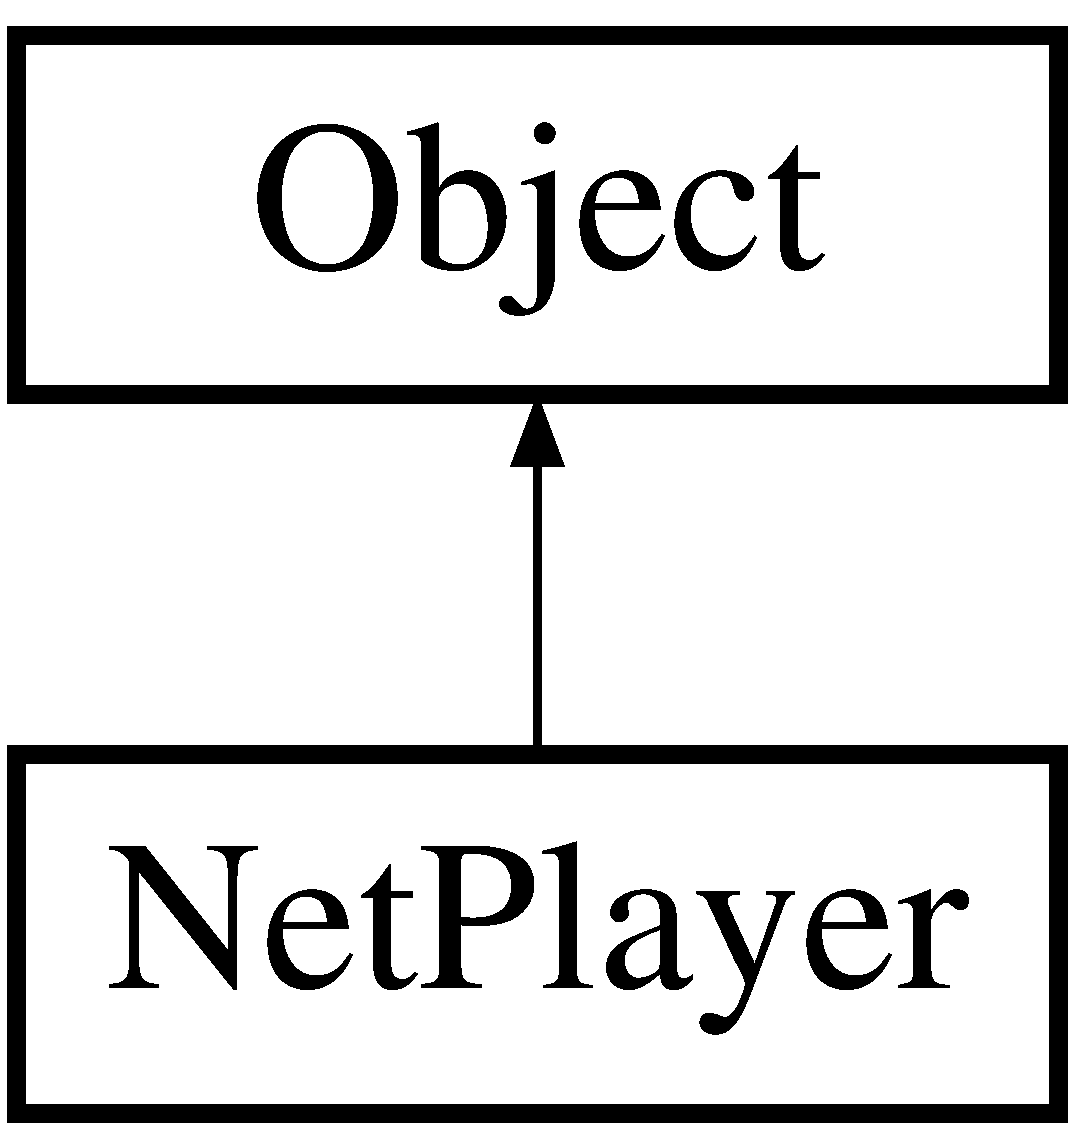
\includegraphics[height=2.000000cm]{class_net_player}
\end{center}
\end{figure}
\subsection*{Public Member Functions}
\begin{DoxyCompactItemize}
\item 
\mbox{\Hypertarget{class_net_player_a8d1c3511be6810041f9edfe8cc2a4550}\label{class_net_player_a8d1c3511be6810041f9edfe8cc2a4550}} 
\hyperlink{class_net_player_a8d1c3511be6810041f9edfe8cc2a4550}{$\sim$\+Net\+Player} ()
\begin{DoxyCompactList}\small\item\em Destructor. \end{DoxyCompactList}\item 
\mbox{\Hypertarget{class_net_player_a830c7ea1d195ca6b8da102db00ebd1d7}\label{class_net_player_a830c7ea1d195ca6b8da102db00ebd1d7}} 
\hyperlink{class_net_player_a830c7ea1d195ca6b8da102db00ebd1d7}{Net\+Player} (\hyperlink{struct_vec2}{Vec2} position, \hyperlink{struct_vec2}{Vec2} scale, Body\+Type type, float32 density, float32 friction, char $\ast$texture, \hyperlink{struct_vec2}{Vec2} sprite\+Origin)
\begin{DoxyCompactList}\small\item\em Constructor. \end{DoxyCompactList}\item 
\mbox{\Hypertarget{class_net_player_aeef1b9ebfac0f5cdd926a616a8988ed5}\label{class_net_player_aeef1b9ebfac0f5cdd926a616a8988ed5}} 
virtual void \hyperlink{class_net_player_aeef1b9ebfac0f5cdd926a616a8988ed5}{Init} () override
\begin{DoxyCompactList}\small\item\em Init. \end{DoxyCompactList}\item 
\mbox{\Hypertarget{class_net_player_a098fab3ea015117852b7580c7fcc4efd}\label{class_net_player_a098fab3ea015117852b7580c7fcc4efd}} 
virtual void \hyperlink{class_net_player_a098fab3ea015117852b7580c7fcc4efd}{Input} () override
\begin{DoxyCompactList}\small\item\em Input. \end{DoxyCompactList}\item 
\mbox{\Hypertarget{class_net_player_a1d47538e8a532dfcb0cddfba3f081575}\label{class_net_player_a1d47538e8a532dfcb0cddfba3f081575}} 
virtual void \hyperlink{class_net_player_a1d47538e8a532dfcb0cddfba3f081575}{Update} () override
\begin{DoxyCompactList}\small\item\em Update. \end{DoxyCompactList}\item 
\mbox{\Hypertarget{class_net_player_ac07584f3a2ece47815aaa863567865cf}\label{class_net_player_ac07584f3a2ece47815aaa863567865cf}} 
virtual Define\+Type \hyperlink{class_net_player_ac07584f3a2ece47815aaa863567865cf}{get\+Define\+Type} () override
\begin{DoxyCompactList}\small\item\em Type of object. \end{DoxyCompactList}\end{DoxyCompactItemize}
\subsection*{Private Attributes}
\begin{DoxyCompactItemize}
\item 
\mbox{\Hypertarget{class_net_player_ac5eef0177a8500703903df1280834d67}\label{class_net_player_ac5eef0177a8500703903df1280834d67}} 
int \hyperlink{class_net_player_ac5eef0177a8500703903df1280834d67}{Index}
\begin{DoxyCompactList}\small\item\em Controls number of players. \end{DoxyCompactList}\end{DoxyCompactItemize}
\subsection*{Additional Inherited Members}


The documentation for this class was generated from the following file\+:\begin{DoxyCompactItemize}
\item 
D\+:/\+Multiplayer/include/netplayer.\+h\end{DoxyCompactItemize}

\hypertarget{class_net_work_manager}{}\section{Net\+Work\+Manager Class Reference}
\label{class_net_work_manager}\index{Net\+Work\+Manager@{Net\+Work\+Manager}}
\subsection*{Public Member Functions}
\begin{DoxyCompactItemize}
\item 
\mbox{\Hypertarget{class_net_work_manager_a3af3630c2f0595dde7968a8343ef2518}\label{class_net_work_manager_a3af3630c2f0595dde7968a8343ef2518}} 
\hyperlink{class_net_work_manager_a3af3630c2f0595dde7968a8343ef2518}{$\sim$\+Net\+Work\+Manager} ()
\begin{DoxyCompactList}\small\item\em Destructor. \end{DoxyCompactList}\item 
bool \hyperlink{class_net_work_manager_ae6aebea892bd72e57ce9e796d7068114}{Connect} (const char $\ast$inserted\+IP, const char $\ast$username, const char $\ast$password)
\item 
\mbox{\Hypertarget{class_net_work_manager_af2f7b5173c1beeab56e115f48b7363bf}\label{class_net_work_manager_af2f7b5173c1beeab56e115f48b7363bf}} 
void \hyperlink{class_net_work_manager_af2f7b5173c1beeab56e115f48b7363bf}{Send\+Game\+Info\+T\+CP} (\hyperlink{struct_coin_info}{Coin\+Info} $\ast$info)
\begin{DoxyCompactList}\small\item\em Send Game information (T\+CP). \end{DoxyCompactList}\item 
\mbox{\Hypertarget{class_net_work_manager_add871151fce653f873aff9ee3f79844e}\label{class_net_work_manager_add871151fce653f873aff9ee3f79844e}} 
void \hyperlink{class_net_work_manager_add871151fce653f873aff9ee3f79844e}{Send\+Player\+Info\+U\+DP} (\hyperlink{struct_player_info}{Player\+Info} $\ast$info)
\begin{DoxyCompactList}\small\item\em Send \hyperlink{class_player}{Player} information (U\+DP). \end{DoxyCompactList}\item 
\mbox{\Hypertarget{class_net_work_manager_a8c5f0058427dffc0a83d2638e1047243}\label{class_net_work_manager_a8c5f0058427dffc0a83d2638e1047243}} 
void \hyperlink{class_net_work_manager_a8c5f0058427dffc0a83d2638e1047243}{Send\+Spike\+Box\+Info\+U\+DP} (\hyperlink{struct_spike_box_info}{Spike\+Box\+Info} $\ast$info)
\begin{DoxyCompactList}\small\item\em Send \hyperlink{class_spike_box}{Spike\+Box} information (U\+DP). \end{DoxyCompactList}\item 
\mbox{\Hypertarget{class_net_work_manager_aed5d68e613999bb570c0509ca8038809}\label{class_net_work_manager_aed5d68e613999bb570c0509ca8038809}} 
void \hyperlink{class_net_work_manager_aed5d68e613999bb570c0509ca8038809}{Send\+Victory\+U\+DP} ()
\begin{DoxyCompactList}\small\item\em Send if someone wins (U\+DP). \end{DoxyCompactList}\item 
\mbox{\Hypertarget{class_net_work_manager_a67c1538c5f1a8380ffaff311564dcd1c}\label{class_net_work_manager_a67c1538c5f1a8380ffaff311564dcd1c}} 
bool \hyperlink{class_net_work_manager_a67c1538c5f1a8380ffaff311564dcd1c}{Receive\+Game\+Info\+T\+CP} ()
\begin{DoxyCompactList}\small\item\em Receive game information (T\+CP). \end{DoxyCompactList}\item 
\mbox{\Hypertarget{class_net_work_manager_af11e307eec500d888e41545fd09c4ccf}\label{class_net_work_manager_af11e307eec500d888e41545fd09c4ccf}} 
void \hyperlink{class_net_work_manager_af11e307eec500d888e41545fd09c4ccf}{Receive\+Game\+Info\+U\+DP} ()
\begin{DoxyCompactList}\small\item\em Receive information (U\+DP) \end{DoxyCompactList}\item 
\mbox{\Hypertarget{class_net_work_manager_a7ade75edb55c3726998d3d30e8c8fead}\label{class_net_work_manager_a7ade75edb55c3726998d3d30e8c8fead}} 
void \hyperlink{class_net_work_manager_a7ade75edb55c3726998d3d30e8c8fead}{Disconnect} ()
\begin{DoxyCompactList}\small\item\em Disconnect. \end{DoxyCompactList}\item 
\mbox{\Hypertarget{class_net_work_manager_a2dfa1d0f5846f68929986367afb2f27d}\label{class_net_work_manager_a2dfa1d0f5846f68929986367afb2f27d}} 
int \hyperlink{class_net_work_manager_a2dfa1d0f5846f68929986367afb2f27d}{Get\+Points} ()
\begin{DoxyCompactList}\small\item\em Get points. \end{DoxyCompactList}\item 
\mbox{\Hypertarget{class_net_work_manager_adc717828d724dd237570783ae810285d}\label{class_net_work_manager_adc717828d724dd237570783ae810285d}} 
void \hyperlink{class_net_work_manager_adc717828d724dd237570783ae810285d}{Set\+Points} (int points)
\begin{DoxyCompactList}\small\item\em Set points. \end{DoxyCompactList}\item 
\mbox{\Hypertarget{class_net_work_manager_aaa905d23fb51701037a374761b6f629e}\label{class_net_work_manager_aaa905d23fb51701037a374761b6f629e}} 
void \hyperlink{class_net_work_manager_aaa905d23fb51701037a374761b6f629e}{Add\+Points} (int points)
\begin{DoxyCompactList}\small\item\em Add points. \end{DoxyCompactList}\item 
\mbox{\Hypertarget{class_net_work_manager_afb82cb5c66b06b0d0ed07d5b816e2531}\label{class_net_work_manager_afb82cb5c66b06b0d0ed07d5b816e2531}} 
void \hyperlink{class_net_work_manager_afb82cb5c66b06b0d0ed07d5b816e2531}{Subtract\+Points} (int points)
\begin{DoxyCompactList}\small\item\em Subtact points. \end{DoxyCompactList}\end{DoxyCompactItemize}
\subsection*{Static Public Member Functions}
\begin{DoxyCompactItemize}
\item 
\mbox{\Hypertarget{class_net_work_manager_ad2c1d65fe860b96f27cd754618740654}\label{class_net_work_manager_ad2c1d65fe860b96f27cd754618740654}} 
static \hyperlink{class_net_work_manager}{Net\+Work\+Manager} $\ast$ \hyperlink{class_net_work_manager_ad2c1d65fe860b96f27cd754618740654}{Get\+Instance} ()
\begin{DoxyCompactList}\small\item\em Get Instance. \end{DoxyCompactList}\end{DoxyCompactItemize}
\subsection*{Public Attributes}
\begin{DoxyCompactItemize}
\item 
\mbox{\Hypertarget{class_net_work_manager_ad7107f1381e38cdddca15fc9bd34c7d0}\label{class_net_work_manager_ad7107f1381e38cdddca15fc9bd34c7d0}} 
\hyperlink{struct_player_info}{Player\+Info} \hyperlink{class_net_work_manager_ad7107f1381e38cdddca15fc9bd34c7d0}{Players} \mbox{[}4\mbox{]}
\begin{DoxyCompactList}\small\item\em Struct declaration that contains all the information that the players need. \end{DoxyCompactList}\item 
\mbox{\Hypertarget{class_net_work_manager_ae7f40c6dc097fbffaaa529ecd634c15b}\label{class_net_work_manager_ae7f40c6dc097fbffaaa529ecd634c15b}} 
\hyperlink{struct_coin_info}{Coin\+Info} \hyperlink{class_net_work_manager_ae7f40c6dc097fbffaaa529ecd634c15b}{Coin}
\begin{DoxyCompactList}\small\item\em Struct declaration that contains all the information that the coins need. \end{DoxyCompactList}\item 
\mbox{\Hypertarget{class_net_work_manager_a1a061b856e3ff9873809adb8689f716d}\label{class_net_work_manager_a1a061b856e3ff9873809adb8689f716d}} 
\hyperlink{struct_spike_box_info}{Spike\+Box\+Info} \hyperlink{class_net_work_manager_a1a061b856e3ff9873809adb8689f716d}{Spike\+Box}
\begin{DoxyCompactList}\small\item\em Struct declaration that contains all the information that the \hyperlink{class_spike_box}{Spike\+Box} need. \end{DoxyCompactList}\item 
\mbox{\Hypertarget{class_net_work_manager_a0bead5f17fd244e7a97c49f1cd081ba5}\label{class_net_work_manager_a0bead5f17fd244e7a97c49f1cd081ba5}} 
Type\+Information \hyperlink{class_net_work_manager_a0bead5f17fd244e7a97c49f1cd081ba5}{Information}
\begin{DoxyCompactList}\small\item\em Struct declaration that contains what type of information it is going to be. \end{DoxyCompactList}\item 
\mbox{\Hypertarget{class_net_work_manager_aca3e5694b6645ef38d28b00a66e226a3}\label{class_net_work_manager_aca3e5694b6645ef38d28b00a66e226a3}} 
int \hyperlink{class_net_work_manager_aca3e5694b6645ef38d28b00a66e226a3}{Player\+Index} = 0
\begin{DoxyCompactList}\small\item\em \hyperlink{class_player}{Player} Index. \end{DoxyCompactList}\end{DoxyCompactItemize}
\subsection*{Private Member Functions}
\begin{DoxyCompactItemize}
\item 
\mbox{\Hypertarget{class_net_work_manager_ae09c43f9bd232bf8a8edb79e0c7f8dac}\label{class_net_work_manager_ae09c43f9bd232bf8a8edb79e0c7f8dac}} 
\hyperlink{class_net_work_manager_ae09c43f9bd232bf8a8edb79e0c7f8dac}{Net\+Work\+Manager} ()
\begin{DoxyCompactList}\small\item\em Constructor. \end{DoxyCompactList}\end{DoxyCompactItemize}
\subsection*{Private Attributes}
\begin{DoxyCompactItemize}
\item 
\mbox{\Hypertarget{class_net_work_manager_a21fb0d7dcdd1caa5c0029ee6dc4b33f5}\label{class_net_work_manager_a21fb0d7dcdd1caa5c0029ee6dc4b33f5}} 
sf\+::\+Tcp\+Socket \hyperlink{class_net_work_manager_a21fb0d7dcdd1caa5c0029ee6dc4b33f5}{T\+C\+P\+Socket}
\begin{DoxyCompactList}\small\item\em T\+CP Socket. \end{DoxyCompactList}\item 
\mbox{\Hypertarget{class_net_work_manager_a462c9099c879257642caa46654320b48}\label{class_net_work_manager_a462c9099c879257642caa46654320b48}} 
sf\+::\+Udp\+Socket \hyperlink{class_net_work_manager_a462c9099c879257642caa46654320b48}{U\+D\+P\+Socket}
\begin{DoxyCompactList}\small\item\em U\+DP Socket. \end{DoxyCompactList}\item 
\mbox{\Hypertarget{class_net_work_manager_a19db3335e4328c5c01dcbbd22346d7a1}\label{class_net_work_manager_a19db3335e4328c5c01dcbbd22346d7a1}} 
const char $\ast$ \hyperlink{class_net_work_manager_a19db3335e4328c5c01dcbbd22346d7a1}{IP}
\begin{DoxyCompactList}\small\item\em IP. \end{DoxyCompactList}\item 
\mbox{\Hypertarget{class_net_work_manager_ae6884c66c9b8e852b1eb974a87d61bdd}\label{class_net_work_manager_ae6884c66c9b8e852b1eb974a87d61bdd}} 
int \hyperlink{class_net_work_manager_ae6884c66c9b8e852b1eb974a87d61bdd}{Points} = 0
\begin{DoxyCompactList}\small\item\em Points. \end{DoxyCompactList}\item 
\mbox{\Hypertarget{class_net_work_manager_ae3b93f01ede6a3bfc23a760672fad965}\label{class_net_work_manager_ae3b93f01ede6a3bfc23a760672fad965}} 
std\+::string \hyperlink{class_net_work_manager_ae3b93f01ede6a3bfc23a760672fad965}{name}
\begin{DoxyCompactList}\small\item\em Username name. \end{DoxyCompactList}\end{DoxyCompactItemize}
\subsection*{Static Private Attributes}
\begin{DoxyCompactItemize}
\item 
\mbox{\Hypertarget{class_net_work_manager_a5b180de3c5674bf1125342f563645243}\label{class_net_work_manager_a5b180de3c5674bf1125342f563645243}} 
static \hyperlink{class_net_work_manager}{Net\+Work\+Manager} $\ast$ \hyperlink{class_net_work_manager_a5b180de3c5674bf1125342f563645243}{Instance}
\begin{DoxyCompactList}\small\item\em Instance. \end{DoxyCompactList}\end{DoxyCompactItemize}


\subsection{Member Function Documentation}
\mbox{\Hypertarget{class_net_work_manager_ae6aebea892bd72e57ce9e796d7068114}\label{class_net_work_manager_ae6aebea892bd72e57ce9e796d7068114}} 
\index{Net\+Work\+Manager@{Net\+Work\+Manager}!Connect@{Connect}}
\index{Connect@{Connect}!Net\+Work\+Manager@{Net\+Work\+Manager}}
\subsubsection{\texorpdfstring{Connect()}{Connect()}}
{\footnotesize\ttfamily bool Net\+Work\+Manager\+::\+Connect (\begin{DoxyParamCaption}\item[{const char $\ast$}]{inserted\+IP,  }\item[{const char $\ast$}]{username,  }\item[{const char $\ast$}]{password }\end{DoxyParamCaption})}

Connect to the game. 
\begin{DoxyParams}{Parameters}
{\em inserted\+IP} & IP. \\
\hline
{\em username} & Username. \\
\hline
{\em password} & Password. \\
\hline
\end{DoxyParams}
\begin{DoxyReturn}{Returns}
The path. 
\end{DoxyReturn}


The documentation for this class was generated from the following file\+:\begin{DoxyCompactItemize}
\item 
D\+:/\+Multiplayer/include/networkmanager.\+h\end{DoxyCompactItemize}

\hypertarget{class_object}{}\section{Object Class Reference}
\label{class_object}\index{Object@{Object}}
Inheritance diagram for Object\+:\begin{figure}[H]
\begin{center}
\leavevmode
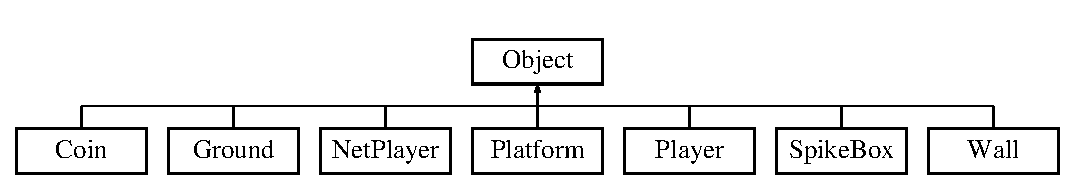
\includegraphics[height=2.000000cm]{class_object}
\end{center}
\end{figure}
\subsection*{Public Member Functions}
\begin{DoxyCompactItemize}
\item 
\mbox{\Hypertarget{class_object_afc4b53523e4e9eb092779843a27268b7}\label{class_object_afc4b53523e4e9eb092779843a27268b7}} 
\hyperlink{class_object_afc4b53523e4e9eb092779843a27268b7}{Object} (\hyperlink{struct_vec2}{Vec2} position, \hyperlink{struct_vec2}{Vec2} scale, Body\+Type type, float32 density, float32 friction, char $\ast$texture, \hyperlink{struct_vec2}{Vec2} sprite\+Origin)
\begin{DoxyCompactList}\small\item\em Desstructor. \end{DoxyCompactList}\item 
\mbox{\Hypertarget{class_object_ae8f5483f459e46687bd01e6f9977afd3}\label{class_object_ae8f5483f459e46687bd01e6f9977afd3}} 
\hyperlink{class_object_ae8f5483f459e46687bd01e6f9977afd3}{$\sim$\+Object} ()
\begin{DoxyCompactList}\small\item\em Constructor. \end{DoxyCompactList}\item 
\mbox{\Hypertarget{class_object_a6e723beba2c9606ab36f1f3674a9537b}\label{class_object_a6e723beba2c9606ab36f1f3674a9537b}} 
virtual void \hyperlink{class_object_a6e723beba2c9606ab36f1f3674a9537b}{Init} ()
\begin{DoxyCompactList}\small\item\em Init. \end{DoxyCompactList}\item 
\mbox{\Hypertarget{class_object_a5a3159b7d5a34c17b9153d72b92ab86d}\label{class_object_a5a3159b7d5a34c17b9153d72b92ab86d}} 
virtual void \hyperlink{class_object_a5a3159b7d5a34c17b9153d72b92ab86d}{Input} ()
\begin{DoxyCompactList}\small\item\em Input. \end{DoxyCompactList}\item 
\mbox{\Hypertarget{class_object_a43f83b38b0497fed04842e7894751206}\label{class_object_a43f83b38b0497fed04842e7894751206}} 
virtual void \hyperlink{class_object_a43f83b38b0497fed04842e7894751206}{Update} ()
\begin{DoxyCompactList}\small\item\em Update. \end{DoxyCompactList}\item 
\mbox{\Hypertarget{class_object_a0af60ea226dcb885e69483452d34a47a}\label{class_object_a0af60ea226dcb885e69483452d34a47a}} 
virtual void \hyperlink{class_object_a0af60ea226dcb885e69483452d34a47a}{Collision} (\hyperlink{class_object}{Object} $\ast$instigator)
\begin{DoxyCompactList}\small\item\em Collision. \end{DoxyCompactList}\item 
\mbox{\Hypertarget{class_object_a9ebf9ef807739f25a04711b90eb82176}\label{class_object_a9ebf9ef807739f25a04711b90eb82176}} 
virtual Define\+Type \hyperlink{class_object_a9ebf9ef807739f25a04711b90eb82176}{get\+Define\+Type} ()
\begin{DoxyCompactList}\small\item\em Type of \hyperlink{class_object}{Object}. \end{DoxyCompactList}\item 
\mbox{\Hypertarget{class_object_ad0c9d66295332df63702940065dbe029}\label{class_object_ad0c9d66295332df63702940065dbe029}} 
virtual void \hyperlink{class_object_ad0c9d66295332df63702940065dbe029}{Reset} ()
\begin{DoxyCompactList}\small\item\em Reset. \end{DoxyCompactList}\item 
\mbox{\Hypertarget{class_object_a2199afbf2f52ff746c4c871e434ff20f}\label{class_object_a2199afbf2f52ff746c4c871e434ff20f}} 
void \hyperlink{class_object_a2199afbf2f52ff746c4c871e434ff20f}{Render} ()
\begin{DoxyCompactList}\small\item\em Render. \end{DoxyCompactList}\end{DoxyCompactItemize}
\subsection*{Public Attributes}
\begin{DoxyCompactItemize}
\item 
\mbox{\Hypertarget{class_object_a629453451f52924956cf615606a59471}\label{class_object_a629453451f52924956cf615606a59471}} 
b2\+Body $\ast$ \hyperlink{class_object_a629453451f52924956cf615606a59471}{Body}
\begin{DoxyCompactList}\small\item\em Body. \end{DoxyCompactList}\end{DoxyCompactItemize}
\subsection*{Protected Member Functions}
\begin{DoxyCompactItemize}
\item 
\mbox{\Hypertarget{class_object_aba86413210bc4e303fde370cad8ab9fe}\label{class_object_aba86413210bc4e303fde370cad8ab9fe}} 
\hyperlink{struct_vec2}{Vec2} \hyperlink{class_object_aba86413210bc4e303fde370cad8ab9fe}{Get\+Position} ()
\begin{DoxyCompactList}\small\item\em Get Position. \end{DoxyCompactList}\item 
\mbox{\Hypertarget{class_object_a24a504120a478e781b9a8128720f8770}\label{class_object_a24a504120a478e781b9a8128720f8770}} 
float32 \hyperlink{class_object_a24a504120a478e781b9a8128720f8770}{Get\+Rotation} ()
\begin{DoxyCompactList}\small\item\em Get Rotation. \end{DoxyCompactList}\item 
void \hyperlink{class_object_a988d9f95eabf06b573b55ad9bce044f6}{Set\+Position} (\hyperlink{struct_vec2}{Vec2} pos, float32 angle)
\item 
void \hyperlink{class_object_a9d94650613651d0f08c27e5ba64cef8f}{Set\+Rotation} (float32 rot)
\end{DoxyCompactItemize}
\subsection*{Private Attributes}
\begin{DoxyCompactItemize}
\item 
\mbox{\Hypertarget{class_object_a6576de27eb814a84d0d4abd87c5960a6}\label{class_object_a6576de27eb814a84d0d4abd87c5960a6}} 
sf\+::\+Texture \hyperlink{class_object_a6576de27eb814a84d0d4abd87c5960a6}{Texture}
\begin{DoxyCompactList}\small\item\em Texture. \end{DoxyCompactList}\item 
\mbox{\Hypertarget{class_object_ae594af01bacdba53a1080ec5fba7a6ff}\label{class_object_ae594af01bacdba53a1080ec5fba7a6ff}} 
sf\+::\+Sprite \hyperlink{class_object_ae594af01bacdba53a1080ec5fba7a6ff}{Last\+Sprite}
\begin{DoxyCompactList}\small\item\em Sprite. \end{DoxyCompactList}\item 
\mbox{\Hypertarget{class_object_af1a4abf4061dfb1113ea703757b33efe}\label{class_object_af1a4abf4061dfb1113ea703757b33efe}} 
b2\+Vec2 \hyperlink{class_object_af1a4abf4061dfb1113ea703757b33efe}{Sprite\+Origin}
\begin{DoxyCompactList}\small\item\em Position Sprite. \end{DoxyCompactList}\item 
\mbox{\Hypertarget{class_object_abb13fcf3d7eb007673019f304d83c0ce}\label{class_object_abb13fcf3d7eb007673019f304d83c0ce}} 
float32 \hyperlink{class_object_abb13fcf3d7eb007673019f304d83c0ce}{Input\+Value}
\begin{DoxyCompactList}\small\item\em Input. \end{DoxyCompactList}\item 
\mbox{\Hypertarget{class_object_a2c39ecbd711c02cae7408d25a665446f}\label{class_object_a2c39ecbd711c02cae7408d25a665446f}} 
\hyperlink{class_collision_call_back}{Collision\+Call\+Back} \hyperlink{class_object_a2c39ecbd711c02cae7408d25a665446f}{Collision\+Call\+Back}
\begin{DoxyCompactList}\small\item\em Collision Call\+Back. \end{DoxyCompactList}\end{DoxyCompactItemize}


\subsection{Member Function Documentation}
\mbox{\Hypertarget{class_object_a988d9f95eabf06b573b55ad9bce044f6}\label{class_object_a988d9f95eabf06b573b55ad9bce044f6}} 
\index{Object@{Object}!Set\+Position@{Set\+Position}}
\index{Set\+Position@{Set\+Position}!Object@{Object}}
\subsubsection{\texorpdfstring{Set\+Position()}{SetPosition()}}
{\footnotesize\ttfamily void Object\+::\+Set\+Position (\begin{DoxyParamCaption}\item[{\hyperlink{struct_vec2}{Vec2}}]{pos,  }\item[{float32}]{angle }\end{DoxyParamCaption})\hspace{0.3cm}{\ttfamily [protected]}}

Set a position 
\begin{DoxyParams}{Parameters}
{\em pos} & x and y.  angle. \\
\hline
\end{DoxyParams}
\mbox{\Hypertarget{class_object_a9d94650613651d0f08c27e5ba64cef8f}\label{class_object_a9d94650613651d0f08c27e5ba64cef8f}} 
\index{Object@{Object}!Set\+Rotation@{Set\+Rotation}}
\index{Set\+Rotation@{Set\+Rotation}!Object@{Object}}
\subsubsection{\texorpdfstring{Set\+Rotation()}{SetRotation()}}
{\footnotesize\ttfamily void Object\+::\+Set\+Rotation (\begin{DoxyParamCaption}\item[{float32}]{rot }\end{DoxyParamCaption})\hspace{0.3cm}{\ttfamily [inline]}, {\ttfamily [protected]}}

Set a rotation 
\begin{DoxyParams}{Parameters}
{\em rot} & rotation. \\
\hline
\end{DoxyParams}


The documentation for this class was generated from the following file\+:\begin{DoxyCompactItemize}
\item 
D\+:/\+Multiplayer/include/object.\+h\end{DoxyCompactItemize}

\hypertarget{class_platform}{}\section{Platform Class Reference}
\label{class_platform}\index{Platform@{Platform}}
Inheritance diagram for Platform\+:\begin{figure}[H]
\begin{center}
\leavevmode
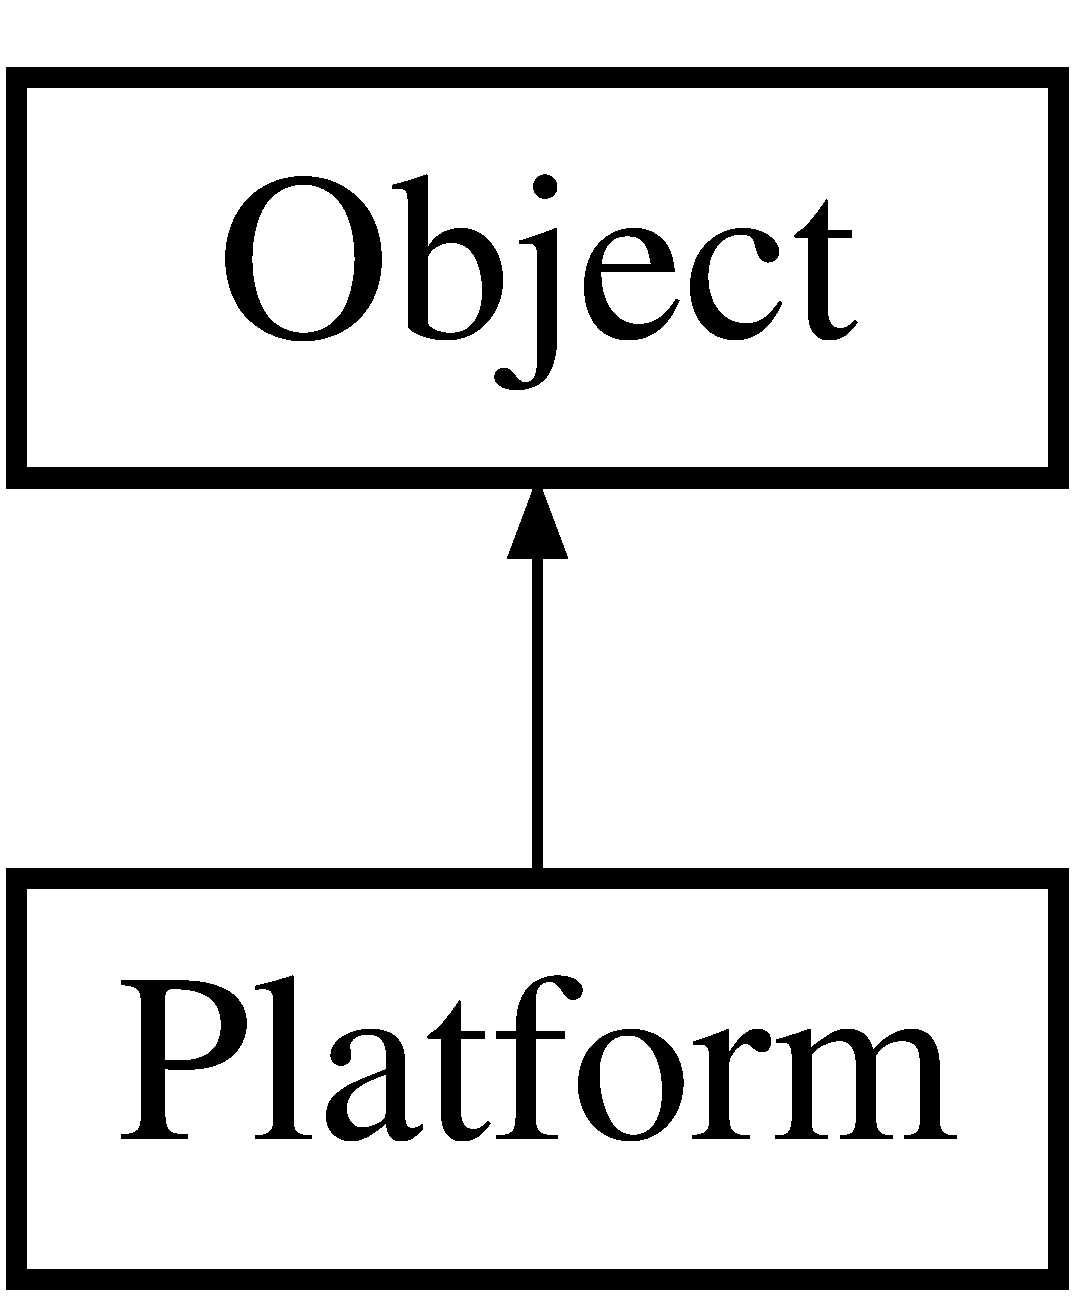
\includegraphics[height=2.000000cm]{class_platform}
\end{center}
\end{figure}
\subsection*{Public Member Functions}
\begin{DoxyCompactItemize}
\item 
\mbox{\Hypertarget{class_platform_a13b5e4ef946b8a2fe38d22014145ab68}\label{class_platform_a13b5e4ef946b8a2fe38d22014145ab68}} 
\hyperlink{class_platform_a13b5e4ef946b8a2fe38d22014145ab68}{$\sim$\+Platform} ()
\begin{DoxyCompactList}\small\item\em Desstructor. \end{DoxyCompactList}\item 
\mbox{\Hypertarget{class_platform_a183e85f66c60e8132fcc039b1d34f2c0}\label{class_platform_a183e85f66c60e8132fcc039b1d34f2c0}} 
\hyperlink{class_platform_a183e85f66c60e8132fcc039b1d34f2c0}{Platform} (\hyperlink{struct_vec2}{Vec2} position, \hyperlink{struct_vec2}{Vec2} scale, Body\+Type type, float32 density, float32 friction, char $\ast$texture, \hyperlink{struct_vec2}{Vec2} sprite\+Origin)
\begin{DoxyCompactList}\small\item\em Constructor. \end{DoxyCompactList}\item 
\mbox{\Hypertarget{class_platform_a25f2e984268e9bf078749e84e7166e61}\label{class_platform_a25f2e984268e9bf078749e84e7166e61}} 
virtual void \hyperlink{class_platform_a25f2e984268e9bf078749e84e7166e61}{Init} () override
\begin{DoxyCompactList}\small\item\em Init. \end{DoxyCompactList}\item 
\mbox{\Hypertarget{class_platform_a4151ba122d6605f575364f4f5bdbf56a}\label{class_platform_a4151ba122d6605f575364f4f5bdbf56a}} 
virtual void \hyperlink{class_platform_a4151ba122d6605f575364f4f5bdbf56a}{Input} () override
\begin{DoxyCompactList}\small\item\em Input. \end{DoxyCompactList}\item 
\mbox{\Hypertarget{class_platform_a97a2696402d99af7f326ed1f238501c3}\label{class_platform_a97a2696402d99af7f326ed1f238501c3}} 
virtual void \hyperlink{class_platform_a97a2696402d99af7f326ed1f238501c3}{Update} () override
\begin{DoxyCompactList}\small\item\em Update. \end{DoxyCompactList}\item 
virtual void \hyperlink{class_platform_abc610ede94941cb4c8423555f8faee13}{Collision} (\hyperlink{class_object}{Object} $\ast$instigator) override
\item 
\mbox{\Hypertarget{class_platform_a4c4b277e82cf60185806779f7bdc01ab}\label{class_platform_a4c4b277e82cf60185806779f7bdc01ab}} 
virtual Define\+Type \hyperlink{class_platform_a4c4b277e82cf60185806779f7bdc01ab}{get\+Define\+Type} () override
\begin{DoxyCompactList}\small\item\em Type of object. \end{DoxyCompactList}\end{DoxyCompactItemize}
\subsection*{Additional Inherited Members}


\subsection{Member Function Documentation}
\mbox{\Hypertarget{class_platform_abc610ede94941cb4c8423555f8faee13}\label{class_platform_abc610ede94941cb4c8423555f8faee13}} 
\index{Platform@{Platform}!Collision@{Collision}}
\index{Collision@{Collision}!Platform@{Platform}}
\subsubsection{\texorpdfstring{Collision()}{Collision()}}
{\footnotesize\ttfamily virtual void Platform\+::\+Collision (\begin{DoxyParamCaption}\item[{\hyperlink{class_object}{Object} $\ast$}]{instigator }\end{DoxyParamCaption})\hspace{0.3cm}{\ttfamily [inline]}, {\ttfamily [override]}, {\ttfamily [virtual]}}

Collision with other objects 
\begin{DoxyParams}{Parameters}
{\em instigator} & Objects name to collide with. \\
\hline
\end{DoxyParams}


Reimplemented from \hyperlink{class_object_a0af60ea226dcb885e69483452d34a47a}{Object}.



The documentation for this class was generated from the following file\+:\begin{DoxyCompactItemize}
\item 
D\+:/\+Multiplayer/include/platform.\+h\end{DoxyCompactItemize}

\hypertarget{class_player}{}\section{Player Class Reference}
\label{class_player}\index{Player@{Player}}
Inheritance diagram for Player\+:\begin{figure}[H]
\begin{center}
\leavevmode
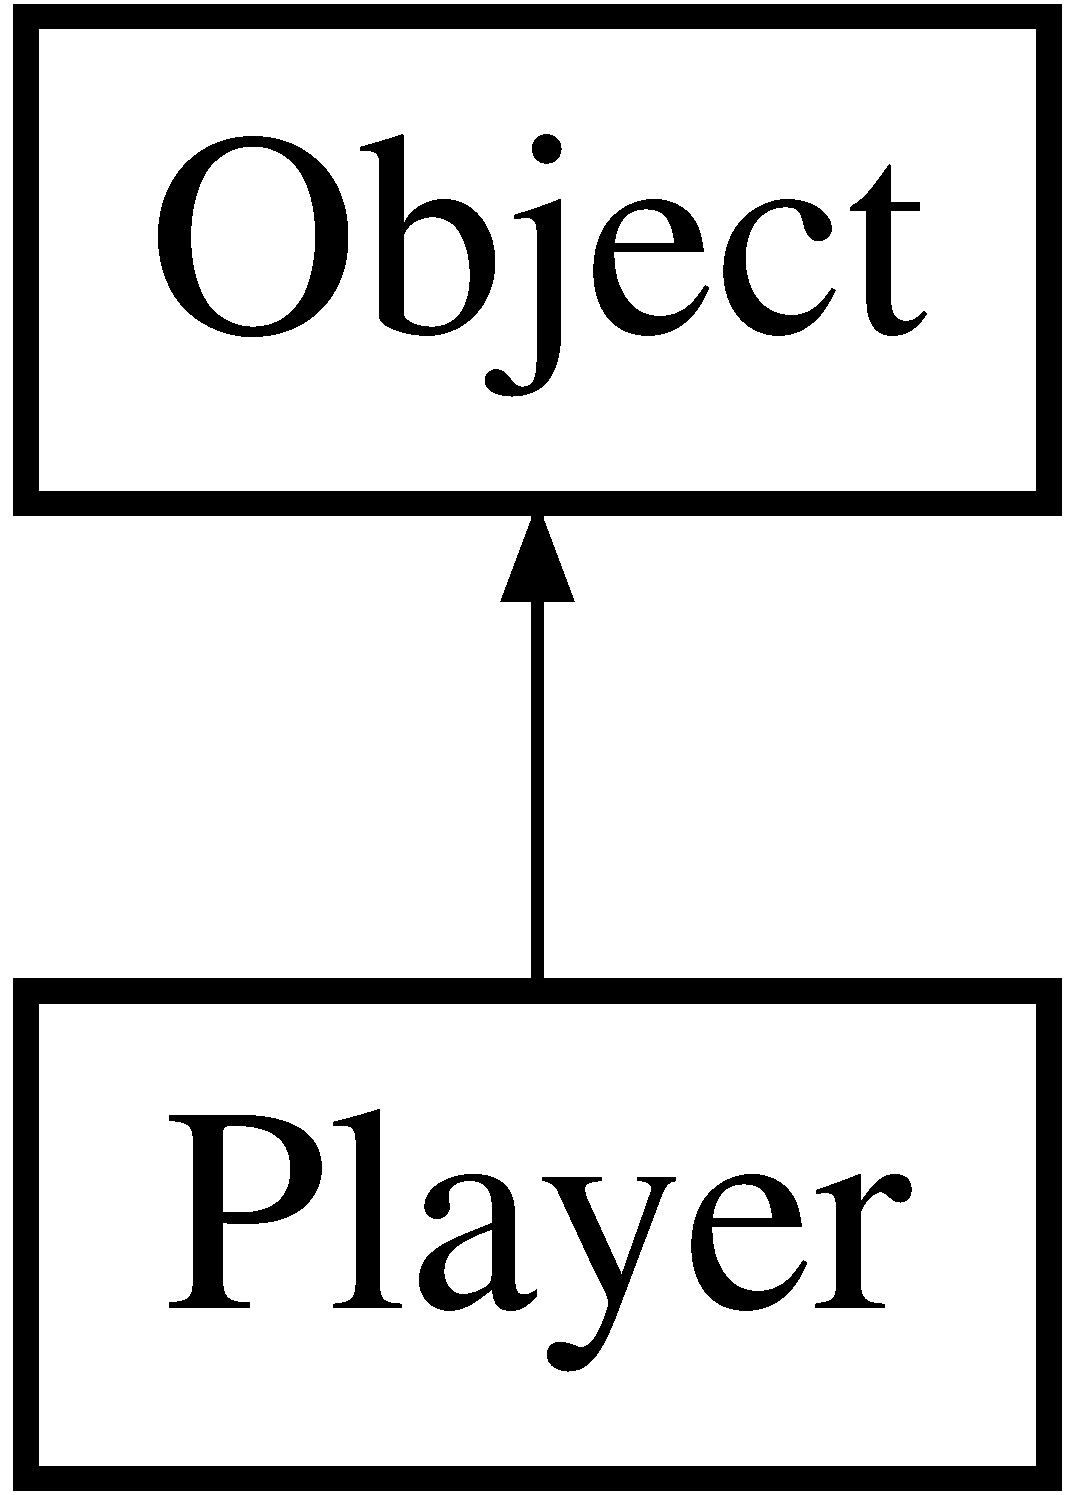
\includegraphics[height=2.000000cm]{class_player}
\end{center}
\end{figure}
\subsection*{Public Member Functions}
\begin{DoxyCompactItemize}
\item 
\mbox{\Hypertarget{class_player_a749d2c00e1fe0f5c2746f7505a58c062}\label{class_player_a749d2c00e1fe0f5c2746f7505a58c062}} 
\hyperlink{class_player_a749d2c00e1fe0f5c2746f7505a58c062}{$\sim$\+Player} ()
\begin{DoxyCompactList}\small\item\em Destructor. \end{DoxyCompactList}\item 
\mbox{\Hypertarget{class_player_a14a4e703b6b79c276ce7ab140f0845ea}\label{class_player_a14a4e703b6b79c276ce7ab140f0845ea}} 
\hyperlink{class_player_a14a4e703b6b79c276ce7ab140f0845ea}{Player} (\hyperlink{struct_vec2}{Vec2} position, \hyperlink{struct_vec2}{Vec2} scale, Body\+Type type, float32 density, float32 friction, char $\ast$texture, \hyperlink{struct_vec2}{Vec2} sprite\+Origin)
\begin{DoxyCompactList}\small\item\em Constructor. \end{DoxyCompactList}\item 
\mbox{\Hypertarget{class_player_af64df6bf1ab0c29d140dd6303262d72f}\label{class_player_af64df6bf1ab0c29d140dd6303262d72f}} 
virtual void \hyperlink{class_player_af64df6bf1ab0c29d140dd6303262d72f}{Init} () override
\begin{DoxyCompactList}\small\item\em Init. \end{DoxyCompactList}\item 
\mbox{\Hypertarget{class_player_a627395e12f5cff3da2c1c9c4395bb0b9}\label{class_player_a627395e12f5cff3da2c1c9c4395bb0b9}} 
virtual void \hyperlink{class_player_a627395e12f5cff3da2c1c9c4395bb0b9}{Input} () override
\begin{DoxyCompactList}\small\item\em Input. \end{DoxyCompactList}\item 
\mbox{\Hypertarget{class_player_a26be3456a62fc667bb4b3adb4ed77233}\label{class_player_a26be3456a62fc667bb4b3adb4ed77233}} 
virtual void \hyperlink{class_player_a26be3456a62fc667bb4b3adb4ed77233}{Update} () override
\begin{DoxyCompactList}\small\item\em Update. \end{DoxyCompactList}\item 
virtual void \hyperlink{class_player_ac2e2422e1637707ed0a032f17392b16b}{Collision} (\hyperlink{class_object}{Object} $\ast$instigator) override
\item 
\mbox{\Hypertarget{class_player_a62d6a7a079668c0881910dc5e1b7b071}\label{class_player_a62d6a7a079668c0881910dc5e1b7b071}} 
virtual void \hyperlink{class_player_a62d6a7a079668c0881910dc5e1b7b071}{Reset} () override
\begin{DoxyCompactList}\small\item\em Reset. \end{DoxyCompactList}\item 
\mbox{\Hypertarget{class_player_a0c74d6bd430490417bb34e9abc233bb7}\label{class_player_a0c74d6bd430490417bb34e9abc233bb7}} 
void \hyperlink{class_player_a0c74d6bd430490417bb34e9abc233bb7}{Kill} ()
\begin{DoxyCompactList}\small\item\em Kill. \end{DoxyCompactList}\item 
\mbox{\Hypertarget{class_player_acdc10d7536a824e02d72d5a5b77875b1}\label{class_player_acdc10d7536a824e02d72d5a5b77875b1}} 
virtual Define\+Type \hyperlink{class_player_acdc10d7536a824e02d72d5a5b77875b1}{get\+Define\+Type} () override
\begin{DoxyCompactList}\small\item\em Type of \hyperlink{class_object}{Object}. \end{DoxyCompactList}\item 
\mbox{\Hypertarget{class_player_a879e5feedffe7445c172968c6084aa54}\label{class_player_a879e5feedffe7445c172968c6084aa54}} 
void \hyperlink{class_player_a879e5feedffe7445c172968c6084aa54}{Disappear} ()
\begin{DoxyCompactList}\small\item\em Disappear if somebody disconnects. \end{DoxyCompactList}\end{DoxyCompactItemize}
\subsection*{Private Attributes}
\begin{DoxyCompactItemize}
\item 
\mbox{\Hypertarget{class_player_a9cd46c1428e2a6fb38916a40ee5ef548}\label{class_player_a9cd46c1428e2a6fb38916a40ee5ef548}} 
bool \hyperlink{class_player_a9cd46c1428e2a6fb38916a40ee5ef548}{Is\+D\+Pressed}
\begin{DoxyCompactList}\small\item\em Is pressing D. \end{DoxyCompactList}\item 
\mbox{\Hypertarget{class_player_a0db9d1d1eca744553f298f9a6b858985}\label{class_player_a0db9d1d1eca744553f298f9a6b858985}} 
bool \hyperlink{class_player_a0db9d1d1eca744553f298f9a6b858985}{Is\+A\+Pressed}
\begin{DoxyCompactList}\small\item\em Is pressing A. \end{DoxyCompactList}\item 
\mbox{\Hypertarget{class_player_ac6445d1f4bc026b52af1b8ce34bb34c1}\label{class_player_ac6445d1f4bc026b52af1b8ce34bb34c1}} 
bool \hyperlink{class_player_ac6445d1f4bc026b52af1b8ce34bb34c1}{Is\+Space\+Pressed}
\begin{DoxyCompactList}\small\item\em Is pressing Space. \end{DoxyCompactList}\item 
\mbox{\Hypertarget{class_player_ac5df350bc9cfeff679e7e47392d120d9}\label{class_player_ac5df350bc9cfeff679e7e47392d120d9}} 
bool \hyperlink{class_player_ac5df350bc9cfeff679e7e47392d120d9}{Is\+Jumping}
\begin{DoxyCompactList}\small\item\em Is pressing Jump. \end{DoxyCompactList}\item 
\mbox{\Hypertarget{class_player_a556019631efc3e7281bd3f9534f23ecd}\label{class_player_a556019631efc3e7281bd3f9534f23ecd}} 
bool \hyperlink{class_player_a556019631efc3e7281bd3f9534f23ecd}{Is\+Killed}
\begin{DoxyCompactList}\small\item\em \hyperlink{class_player}{Player} has been killed. \end{DoxyCompactList}\end{DoxyCompactItemize}
\subsection*{Additional Inherited Members}


\subsection{Member Function Documentation}
\mbox{\Hypertarget{class_player_ac2e2422e1637707ed0a032f17392b16b}\label{class_player_ac2e2422e1637707ed0a032f17392b16b}} 
\index{Player@{Player}!Collision@{Collision}}
\index{Collision@{Collision}!Player@{Player}}
\subsubsection{\texorpdfstring{Collision()}{Collision()}}
{\footnotesize\ttfamily virtual void Player\+::\+Collision (\begin{DoxyParamCaption}\item[{\hyperlink{class_object}{Object} $\ast$}]{instigator }\end{DoxyParamCaption})\hspace{0.3cm}{\ttfamily [override]}, {\ttfamily [virtual]}}

Collision with other objects 
\begin{DoxyParams}{Parameters}
{\em instigator} & Objects name to collide with. \\
\hline
\end{DoxyParams}


Reimplemented from \hyperlink{class_object_a0af60ea226dcb885e69483452d34a47a}{Object}.



The documentation for this class was generated from the following file\+:\begin{DoxyCompactItemize}
\item 
D\+:/\+Multiplayer/include/player.\+h\end{DoxyCompactItemize}

\hypertarget{struct_player_info}{}\section{Player\+Info Struct Reference}
\label{struct_player_info}\index{Player\+Info@{Player\+Info}}


{\ttfamily \#include $<$networkmanager.\+h$>$}

\subsection*{Public Attributes}
\begin{DoxyCompactItemize}
\item 
\mbox{\Hypertarget{struct_player_info_a1a7b2407a8c8e565179951a8e0967017}\label{struct_player_info_a1a7b2407a8c8e565179951a8e0967017}} 
float {\bfseries PosX}
\item 
\mbox{\Hypertarget{struct_player_info_a378eed19a95ececc667970d7a14b8f31}\label{struct_player_info_a378eed19a95ececc667970d7a14b8f31}} 
float {\bfseries PosY}
\item 
\mbox{\Hypertarget{struct_player_info_ab04486c35400ab0dadfcea6bda8dd033}\label{struct_player_info_ab04486c35400ab0dadfcea6bda8dd033}} 
float {\bfseries Rotation}
\item 
\mbox{\Hypertarget{struct_player_info_a0499cbd42d40f45a0e1ae1652bf9b69f}\label{struct_player_info_a0499cbd42d40f45a0e1ae1652bf9b69f}} 
int {\bfseries Points}
\end{DoxyCompactItemize}


\subsection{Detailed Description}
Struct All the information that the player needs to receive and send 

The documentation for this struct was generated from the following file\+:\begin{DoxyCompactItemize}
\item 
D\+:/\+Multiplayer/include/networkmanager.\+h\end{DoxyCompactItemize}

\hypertarget{struct_points_pos_users_text}{}\section{Points\+Pos\+Users\+Text Struct Reference}
\label{struct_points_pos_users_text}\index{Points\+Pos\+Users\+Text@{Points\+Pos\+Users\+Text}}


{\ttfamily \#include $<$scene.\+h$>$}

\subsection*{Public Attributes}
\begin{DoxyCompactItemize}
\item 
\mbox{\Hypertarget{struct_points_pos_users_text_a82324a71c73e0ee06d86db7457cb20c6}\label{struct_points_pos_users_text_a82324a71c73e0ee06d86db7457cb20c6}} 
float {\bfseries PosX}
\item 
\mbox{\Hypertarget{struct_points_pos_users_text_a36c942a28e9e04ffb94a96bc0233dcbb}\label{struct_points_pos_users_text_a36c942a28e9e04ffb94a96bc0233dcbb}} 
float {\bfseries PosY}
\item 
\mbox{\Hypertarget{struct_points_pos_users_text_ae5df179503ec3f1b37eaa1e561fec5e1}\label{struct_points_pos_users_text_ae5df179503ec3f1b37eaa1e561fec5e1}} 
int {\bfseries Points}
\end{DoxyCompactItemize}


\subsection{Detailed Description}
Struct Where to put the text and the number of points on each player 

The documentation for this struct was generated from the following file\+:\begin{DoxyCompactItemize}
\item 
D\+:/\+Multiplayer/include/scene.\+h\end{DoxyCompactItemize}

\hypertarget{class_scene}{}\section{Scene Class Reference}
\label{class_scene}\index{Scene@{Scene}}
\subsection*{Public Member Functions}
\begin{DoxyCompactItemize}
\item 
\mbox{\Hypertarget{class_scene_a3b8cec2e32546713915f8c6303c951f1}\label{class_scene_a3b8cec2e32546713915f8c6303c951f1}} 
\hyperlink{class_scene_a3b8cec2e32546713915f8c6303c951f1}{$\sim$\+Scene} ()
\begin{DoxyCompactList}\small\item\em Desstructor. \end{DoxyCompactList}\item 
\mbox{\Hypertarget{class_scene_a442dd94af5bd4ee544c929832f4eed6a}\label{class_scene_a442dd94af5bd4ee544c929832f4eed6a}} 
Scene\+Type \hyperlink{class_scene_a442dd94af5bd4ee544c929832f4eed6a}{Get\+Scene} ()
\begin{DoxyCompactList}\small\item\em Get scene. \end{DoxyCompactList}\item 
\mbox{\Hypertarget{class_scene_a2c78bfa591688e99f314a5f193c6c4f0}\label{class_scene_a2c78bfa591688e99f314a5f193c6c4f0}} 
void \hyperlink{class_scene_a2c78bfa591688e99f314a5f193c6c4f0}{Set\+Scene} (Scene\+Type scene)
\begin{DoxyCompactList}\small\item\em Set scene. \end{DoxyCompactList}\item 
\mbox{\Hypertarget{class_scene_ae0de17df8ca6fd97d47824be1f9e7634}\label{class_scene_ae0de17df8ca6fd97d47824be1f9e7634}} 
sf\+::\+Text \hyperlink{class_scene_ae0de17df8ca6fd97d47824be1f9e7634}{Get\+Score\+Text} ()
\begin{DoxyCompactList}\small\item\em Get score text. \end{DoxyCompactList}\item 
\mbox{\Hypertarget{class_scene_a59803cc75dca996bd66d6acdaa99df76}\label{class_scene_a59803cc75dca996bd66d6acdaa99df76}} 
sf\+::\+Text \hyperlink{class_scene_a59803cc75dca996bd66d6acdaa99df76}{Get\+Points} ()
\begin{DoxyCompactList}\small\item\em Get points text. \end{DoxyCompactList}\item 
\mbox{\Hypertarget{class_scene_afabdeb9a701ec252fe30e9da5b112f28}\label{class_scene_afabdeb9a701ec252fe30e9da5b112f28}} 
sf\+::\+Text \hyperlink{class_scene_afabdeb9a701ec252fe30e9da5b112f28}{Get\+Game\+Over\+Title} ()
\begin{DoxyCompactList}\small\item\em Get game over title text. \end{DoxyCompactList}\item 
\mbox{\Hypertarget{class_scene_a798247e1af7411704abbc1ff37e3cc90}\label{class_scene_a798247e1af7411704abbc1ff37e3cc90}} 
sf\+::\+Text \hyperlink{class_scene_a798247e1af7411704abbc1ff37e3cc90}{Get\+Game\+Over\+Win\+Text} ()
\begin{DoxyCompactList}\small\item\em Get game over win text. \end{DoxyCompactList}\item 
\mbox{\Hypertarget{class_scene_af4e7a704107a6a2a2f2fc272b74e9c7a}\label{class_scene_af4e7a704107a6a2a2f2fc272b74e9c7a}} 
sf\+::\+Text \hyperlink{class_scene_af4e7a704107a6a2a2f2fc272b74e9c7a}{Get\+Game\+Over\+Winner\+Name\+Text} ()
\begin{DoxyCompactList}\small\item\em Get game over winner name text. \end{DoxyCompactList}\item 
\mbox{\Hypertarget{class_scene_a914f803fcc95618fb7b30ce67ec7da43}\label{class_scene_a914f803fcc95618fb7b30ce67ec7da43}} 
sf\+::\+Text \hyperlink{class_scene_a914f803fcc95618fb7b30ce67ec7da43}{Get\+Game\+Over\+Congratulations\+Text} ()
\begin{DoxyCompactList}\small\item\em Get game over congratulations text. \end{DoxyCompactList}\item 
\mbox{\Hypertarget{class_scene_ac0459bb78a21a66f041f1d2ca4be2180}\label{class_scene_ac0459bb78a21a66f041f1d2ca4be2180}} 
sf\+::\+Text \hyperlink{class_scene_ac0459bb78a21a66f041f1d2ca4be2180}{Get\+Game\+Over\+Lose\+Text} ()
\begin{DoxyCompactList}\small\item\em Get game over lose text. \end{DoxyCompactList}\item 
\mbox{\Hypertarget{class_scene_aa2edffc8f2f4a04b033e4ee9f46fb618}\label{class_scene_aa2edffc8f2f4a04b033e4ee9f46fb618}} 
sf\+::\+Text \hyperlink{class_scene_aa2edffc8f2f4a04b033e4ee9f46fb618}{Get\+Game\+Over\+Loser\+Name\+Text} ()
\begin{DoxyCompactList}\small\item\em Get game over loser name text. \end{DoxyCompactList}\item 
\mbox{\Hypertarget{class_scene_a783b5b7ba01a4acc1484cc1536c7ecd8}\label{class_scene_a783b5b7ba01a4acc1484cc1536c7ecd8}} 
sf\+::\+Text \hyperlink{class_scene_a783b5b7ba01a4acc1484cc1536c7ecd8}{Get\+Game\+Over\+Lose\+Winner\+Text} ()
\begin{DoxyCompactList}\small\item\em Get game over loser winner text. \end{DoxyCompactList}\item 
\mbox{\Hypertarget{class_scene_ae0e6d7336865ab34f7bf7dfcfbf7ec8a}\label{class_scene_ae0e6d7336865ab34f7bf7dfcfbf7ec8a}} 
sf\+::\+Text \hyperlink{class_scene_ae0e6d7336865ab34f7bf7dfcfbf7ec8a}{Get\+In\+Game\+Name\+Text} ()
\begin{DoxyCompactList}\small\item\em Get in game name text. \end{DoxyCompactList}\item 
\mbox{\Hypertarget{class_scene_a6310c6c3e49cee3e2a95b2348a502411}\label{class_scene_a6310c6c3e49cee3e2a95b2348a502411}} 
sf\+::\+Text \hyperlink{class_scene_a6310c6c3e49cee3e2a95b2348a502411}{Get\+In\+Game\+Other\+Users\+Points\+Text1} ()
\begin{DoxyCompactList}\small\item\em Get in game other users points text;. \end{DoxyCompactList}\item 
\mbox{\Hypertarget{class_scene_a7ca8a4fd01af145d9bdf159832aeb7a6}\label{class_scene_a7ca8a4fd01af145d9bdf159832aeb7a6}} 
sf\+::\+Text \hyperlink{class_scene_a7ca8a4fd01af145d9bdf159832aeb7a6}{Get\+In\+Game\+Other\+Users\+Points\+Text2} ()
\begin{DoxyCompactList}\small\item\em Get in game other users points 2 text;. \end{DoxyCompactList}\item 
\mbox{\Hypertarget{class_scene_aef2f52b7403879bf76ddb4d614249960}\label{class_scene_aef2f52b7403879bf76ddb4d614249960}} 
sf\+::\+Text \hyperlink{class_scene_aef2f52b7403879bf76ddb4d614249960}{Get\+In\+Game\+Other\+Users\+Points\+Text3} ()
\begin{DoxyCompactList}\small\item\em Get in game other users points 3 text;. \end{DoxyCompactList}\item 
\mbox{\Hypertarget{class_scene_ad0dd362ee307861e9172d82e9743056e}\label{class_scene_ad0dd362ee307861e9172d82e9743056e}} 
sf\+::\+Text \hyperlink{class_scene_ad0dd362ee307861e9172d82e9743056e}{Get\+In\+Game\+Other\+Users\+Points\+Text4} ()
\begin{DoxyCompactList}\small\item\em Get in game other users points 4 text;. \end{DoxyCompactList}\item 
\mbox{\Hypertarget{class_scene_ac15d67d5b428ba39750e5f93e823b285}\label{class_scene_ac15d67d5b428ba39750e5f93e823b285}} 
std\+::string \hyperlink{class_scene_ac15d67d5b428ba39750e5f93e823b285}{Get\+Game\+Over\+Win\+Name} ()
\begin{DoxyCompactList}\small\item\em Get game over win name. \end{DoxyCompactList}\item 
\mbox{\Hypertarget{class_scene_aca4047a5eb30c611197068c72a16012d}\label{class_scene_aca4047a5eb30c611197068c72a16012d}} 
void \hyperlink{class_scene_aca4047a5eb30c611197068c72a16012d}{Set\+Game\+Over\+Winner\+Name} (std\+::string name)
\begin{DoxyCompactList}\small\item\em Set game over winner name. \end{DoxyCompactList}\item 
\mbox{\Hypertarget{class_scene_afd80687a6bf3f8324945d8c911986b8f}\label{class_scene_afd80687a6bf3f8324945d8c911986b8f}} 
std\+::string \hyperlink{class_scene_afd80687a6bf3f8324945d8c911986b8f}{Get\+Game\+Over\+Loser\+Name} ()
\begin{DoxyCompactList}\small\item\em Get game over loser name. \end{DoxyCompactList}\item 
\mbox{\Hypertarget{class_scene_a41723bff4fabc191aa28326bbcd6b12c}\label{class_scene_a41723bff4fabc191aa28326bbcd6b12c}} 
void \hyperlink{class_scene_a41723bff4fabc191aa28326bbcd6b12c}{Set\+Game\+Over\+Loser\+Name} (std\+::string name)
\begin{DoxyCompactList}\small\item\em Set game over loser name. \end{DoxyCompactList}\item 
\mbox{\Hypertarget{class_scene_afbedeca41dbcd2afb3d4ad22e42ab5f8}\label{class_scene_afbedeca41dbcd2afb3d4ad22e42ab5f8}} 
void \hyperlink{class_scene_afbedeca41dbcd2afb3d4ad22e42ab5f8}{Set\+In\+Game\+Other\+Users\+Points\+Pos\+XY} (User user, float x, float y, int points)
\begin{DoxyCompactList}\small\item\em Set in game other users points pos x, y and points. \end{DoxyCompactList}\item 
\mbox{\Hypertarget{class_scene_a0ca76b15bf796d518b68403ebd66c872}\label{class_scene_a0ca76b15bf796d518b68403ebd66c872}} 
void \hyperlink{class_scene_a0ca76b15bf796d518b68403ebd66c872}{Check\+Files} ()
\begin{DoxyCompactList}\small\item\em Check if files are running. \end{DoxyCompactList}\item 
\mbox{\Hypertarget{class_scene_a43e948c59bb0e726b0fb91eaabcb1c49}\label{class_scene_a43e948c59bb0e726b0fb91eaabcb1c49}} 
void \hyperlink{class_scene_a43e948c59bb0e726b0fb91eaabcb1c49}{Draw\+Main\+Menu} ()
\begin{DoxyCompactList}\small\item\em Draw Main Menu. \end{DoxyCompactList}\item 
\mbox{\Hypertarget{class_scene_a03e8c212f77c14c9373c4aa490bfc951}\label{class_scene_a03e8c212f77c14c9373c4aa490bfc951}} 
void \hyperlink{class_scene_a03e8c212f77c14c9373c4aa490bfc951}{Input\+Main\+Menu} ()
\begin{DoxyCompactList}\small\item\em Input Main Menu. \end{DoxyCompactList}\item 
\mbox{\Hypertarget{class_scene_a6cfb68f3859836aeeb4b4da8daacb6f9}\label{class_scene_a6cfb68f3859836aeeb4b4da8daacb6f9}} 
void \hyperlink{class_scene_a6cfb68f3859836aeeb4b4da8daacb6f9}{Update\+Main\+Menu} ()
\begin{DoxyCompactList}\small\item\em Update Main Menu. \end{DoxyCompactList}\item 
\mbox{\Hypertarget{class_scene_abcfd2a3bf65339437d0858b185862645}\label{class_scene_abcfd2a3bf65339437d0858b185862645}} 
void \hyperlink{class_scene_abcfd2a3bf65339437d0858b185862645}{Draw\+Game\+Labels} ()
\begin{DoxyCompactList}\small\item\em Draw game labels. \end{DoxyCompactList}\item 
\mbox{\Hypertarget{class_scene_ac6eb6c5125587a6892014c9f780e3c4e}\label{class_scene_ac6eb6c5125587a6892014c9f780e3c4e}} 
void \hyperlink{class_scene_ac6eb6c5125587a6892014c9f780e3c4e}{Update\+Game\+Labels} ()
\begin{DoxyCompactList}\small\item\em Update Game labels. \end{DoxyCompactList}\item 
\mbox{\Hypertarget{class_scene_ad3f5f2c640883175892a7a5de83bfce6}\label{class_scene_ad3f5f2c640883175892a7a5de83bfce6}} 
void \hyperlink{class_scene_ad3f5f2c640883175892a7a5de83bfce6}{Draw\+Game\+Over\+Win} ()
\begin{DoxyCompactList}\small\item\em Draw Game Over Win. \end{DoxyCompactList}\item 
\mbox{\Hypertarget{class_scene_a55a60bb3bef24f519fa4e3fb763d5b4f}\label{class_scene_a55a60bb3bef24f519fa4e3fb763d5b4f}} 
void \hyperlink{class_scene_a55a60bb3bef24f519fa4e3fb763d5b4f}{Draw\+Game\+Over\+Lose} ()
\begin{DoxyCompactList}\small\item\em Draw Game Over Lose. \end{DoxyCompactList}\item 
\mbox{\Hypertarget{class_scene_a97e5de0ca09046583ea6f7732fb8c8cb}\label{class_scene_a97e5de0ca09046583ea6f7732fb8c8cb}} 
void \hyperlink{class_scene_a97e5de0ca09046583ea6f7732fb8c8cb}{Update\+Game\+Over} ()
\begin{DoxyCompactList}\small\item\em Update Game Over. \end{DoxyCompactList}\item 
\mbox{\Hypertarget{class_scene_ae04d616af3648d27068a24ce174a0eb5}\label{class_scene_ae04d616af3648d27068a24ce174a0eb5}} 
void \hyperlink{class_scene_ae04d616af3648d27068a24ce174a0eb5}{Input\+Scene} (Scene\+Type scene)
\begin{DoxyCompactList}\small\item\em Input. \end{DoxyCompactList}\item 
\mbox{\Hypertarget{class_scene_a0b40f7844546047103c7b00066122f90}\label{class_scene_a0b40f7844546047103c7b00066122f90}} 
void \hyperlink{class_scene_a0b40f7844546047103c7b00066122f90}{Update} (Scene\+Type scene)
\begin{DoxyCompactList}\small\item\em Update. \end{DoxyCompactList}\item 
\mbox{\Hypertarget{class_scene_ab102b0a0b0b44de765e2d644051b01e9}\label{class_scene_ab102b0a0b0b44de765e2d644051b01e9}} 
void \hyperlink{class_scene_ab102b0a0b0b44de765e2d644051b01e9}{Draw\+Scene} (Scene\+Type scene)
\begin{DoxyCompactList}\small\item\em Render. \end{DoxyCompactList}\end{DoxyCompactItemize}
\subsection*{Static Public Member Functions}
\begin{DoxyCompactItemize}
\item 
\mbox{\Hypertarget{class_scene_aa0000b4d56229722e7aa8c151ad02a4f}\label{class_scene_aa0000b4d56229722e7aa8c151ad02a4f}} 
static \hyperlink{class_scene}{Scene} $\ast$ \hyperlink{class_scene_aa0000b4d56229722e7aa8c151ad02a4f}{Get\+Instance} ()
\begin{DoxyCompactList}\small\item\em Get instance. \end{DoxyCompactList}\end{DoxyCompactItemize}
\subsection*{Private Member Functions}
\begin{DoxyCompactItemize}
\item 
\mbox{\Hypertarget{class_scene_ad10176d75a9cc0da56626f682d083507}\label{class_scene_ad10176d75a9cc0da56626f682d083507}} 
\hyperlink{class_scene_ad10176d75a9cc0da56626f682d083507}{Scene} ()
\begin{DoxyCompactList}\small\item\em Constructor. \end{DoxyCompactList}\end{DoxyCompactItemize}
\subsection*{Private Attributes}
\begin{DoxyCompactItemize}
\item 
\mbox{\Hypertarget{class_scene_a467663d72eee058248778dafc4742be6}\label{class_scene_a467663d72eee058248778dafc4742be6}} 
Scene\+Type \hyperlink{class_scene_a467663d72eee058248778dafc4742be6}{Current\+Scene}
\begin{DoxyCompactList}\small\item\em Current \hyperlink{class_scene}{Scene}. \end{DoxyCompactList}\item 
\mbox{\Hypertarget{class_scene_af19add9cae49f93cef39707fb76ccf8b}\label{class_scene_af19add9cae49f93cef39707fb76ccf8b}} 
sf\+::\+Font \hyperlink{class_scene_af19add9cae49f93cef39707fb76ccf8b}{Font}
\begin{DoxyCompactList}\small\item\em Font. \end{DoxyCompactList}\item 
\mbox{\Hypertarget{class_scene_a8d628bb089414982afa2255b3e43838d}\label{class_scene_a8d628bb089414982afa2255b3e43838d}} 
sf\+::\+Text \hyperlink{class_scene_a8d628bb089414982afa2255b3e43838d}{Score\+Text}
\begin{DoxyCompactList}\small\item\em Score text. \end{DoxyCompactList}\item 
\mbox{\Hypertarget{class_scene_a9ff9acc70ca85151ee11ffa34f68373e}\label{class_scene_a9ff9acc70ca85151ee11ffa34f68373e}} 
sf\+::\+Text \hyperlink{class_scene_a9ff9acc70ca85151ee11ffa34f68373e}{Points}
\begin{DoxyCompactList}\small\item\em Points text. \end{DoxyCompactList}\item 
\mbox{\Hypertarget{class_scene_a34a041c6e0437c33787c38ed9f3635e2}\label{class_scene_a34a041c6e0437c33787c38ed9f3635e2}} 
sf\+::\+Text \hyperlink{class_scene_a34a041c6e0437c33787c38ed9f3635e2}{Game\+Over\+Title}
\begin{DoxyCompactList}\small\item\em Game\+Over title text. \end{DoxyCompactList}\item 
\mbox{\Hypertarget{class_scene_af3c1d7ed4dfa6d441fe40cffb413eb24}\label{class_scene_af3c1d7ed4dfa6d441fe40cffb413eb24}} 
std\+::string \hyperlink{class_scene_af3c1d7ed4dfa6d441fe40cffb413eb24}{Game\+Over\+Winner\+Name}
\begin{DoxyCompactList}\small\item\em Game\+Over winner name. \end{DoxyCompactList}\item 
\mbox{\Hypertarget{class_scene_a02adffe1edcd7b14435e1876b95e529e}\label{class_scene_a02adffe1edcd7b14435e1876b95e529e}} 
std\+::string \hyperlink{class_scene_a02adffe1edcd7b14435e1876b95e529e}{Game\+Over\+Loser\+Name}
\begin{DoxyCompactList}\small\item\em Game\+Over loser name. \end{DoxyCompactList}\item 
\mbox{\Hypertarget{class_scene_a98ad3f69554feb8b98832b61e921aacd}\label{class_scene_a98ad3f69554feb8b98832b61e921aacd}} 
sf\+::\+Text \hyperlink{class_scene_a98ad3f69554feb8b98832b61e921aacd}{Game\+Over\+Win\+Text}
\begin{DoxyCompactList}\small\item\em Game\+Over win text. \end{DoxyCompactList}\item 
\mbox{\Hypertarget{class_scene_ac188fb7e7b2231a2d5fdc9a694258659}\label{class_scene_ac188fb7e7b2231a2d5fdc9a694258659}} 
sf\+::\+Text \hyperlink{class_scene_ac188fb7e7b2231a2d5fdc9a694258659}{Game\+Over\+Winner\+Name\+Text}
\begin{DoxyCompactList}\small\item\em Game\+Over winner name text. \end{DoxyCompactList}\item 
\mbox{\Hypertarget{class_scene_a44744105b4bcffdb246defaa8ccc8bb1}\label{class_scene_a44744105b4bcffdb246defaa8ccc8bb1}} 
sf\+::\+Text \hyperlink{class_scene_a44744105b4bcffdb246defaa8ccc8bb1}{Game\+Over\+Congratulations\+Text}
\begin{DoxyCompactList}\small\item\em Game\+Over congratulations text. \end{DoxyCompactList}\item 
\mbox{\Hypertarget{class_scene_a5ae0a07930648e894ae5ad08b0a508bf}\label{class_scene_a5ae0a07930648e894ae5ad08b0a508bf}} 
sf\+::\+Text \hyperlink{class_scene_a5ae0a07930648e894ae5ad08b0a508bf}{Game\+Over\+Lose\+Text}
\begin{DoxyCompactList}\small\item\em Game\+Over lose text. \end{DoxyCompactList}\item 
\mbox{\Hypertarget{class_scene_a3bb80209dbb364c2b214114e635f8c43}\label{class_scene_a3bb80209dbb364c2b214114e635f8c43}} 
sf\+::\+Text \hyperlink{class_scene_a3bb80209dbb364c2b214114e635f8c43}{Game\+Over\+Loser\+Name\+Text}
\begin{DoxyCompactList}\small\item\em Game\+Over loser name text. \end{DoxyCompactList}\item 
\mbox{\Hypertarget{class_scene_ad5cd07426583868ba369b9e17b39bf07}\label{class_scene_ad5cd07426583868ba369b9e17b39bf07}} 
sf\+::\+Text \hyperlink{class_scene_ad5cd07426583868ba369b9e17b39bf07}{Game\+Over\+Lose\+Winner\+Text}
\begin{DoxyCompactList}\small\item\em Game\+Over lose winner text. \end{DoxyCompactList}\item 
\mbox{\Hypertarget{class_scene_a5ab29d6ee8177b400174177a61169b5f}\label{class_scene_a5ab29d6ee8177b400174177a61169b5f}} 
sf\+::\+Text \hyperlink{class_scene_a5ab29d6ee8177b400174177a61169b5f}{In\+Game\+Name\+Text}
\begin{DoxyCompactList}\small\item\em In Game Name Text. \end{DoxyCompactList}\item 
\mbox{\Hypertarget{class_scene_a933b81b9c2f1023cbc7a5a07e3f32fc7}\label{class_scene_a933b81b9c2f1023cbc7a5a07e3f32fc7}} 
std\+::string \hyperlink{class_scene_a933b81b9c2f1023cbc7a5a07e3f32fc7}{In\+Game\+Name}
\begin{DoxyCompactList}\small\item\em User Name. \end{DoxyCompactList}\item 
\mbox{\Hypertarget{class_scene_a6fdf0dc1fd4bc12c2bc8933f9e821d45}\label{class_scene_a6fdf0dc1fd4bc12c2bc8933f9e821d45}} 
sf\+::\+Text \hyperlink{class_scene_a6fdf0dc1fd4bc12c2bc8933f9e821d45}{In\+Game\+Other\+Users\+Points\+Text1}
\begin{DoxyCompactList}\small\item\em In Game Other Users Points Text 1. \end{DoxyCompactList}\item 
\mbox{\Hypertarget{class_scene_aed6894b4cb258d6acf8f26d1242f4684}\label{class_scene_aed6894b4cb258d6acf8f26d1242f4684}} 
sf\+::\+Text \hyperlink{class_scene_aed6894b4cb258d6acf8f26d1242f4684}{In\+Game\+Other\+Users\+Points\+Text2}
\begin{DoxyCompactList}\small\item\em In Game Other Users Points Text 2. \end{DoxyCompactList}\item 
\mbox{\Hypertarget{class_scene_af38a4226d50df64037b4d351751fce8c}\label{class_scene_af38a4226d50df64037b4d351751fce8c}} 
sf\+::\+Text \hyperlink{class_scene_af38a4226d50df64037b4d351751fce8c}{In\+Game\+Other\+Users\+Points\+Text3}
\begin{DoxyCompactList}\small\item\em In Game Other Users Points Text 3. \end{DoxyCompactList}\item 
\mbox{\Hypertarget{class_scene_a82027fe8571432fe3548ef410a187e29}\label{class_scene_a82027fe8571432fe3548ef410a187e29}} 
sf\+::\+Text \hyperlink{class_scene_a82027fe8571432fe3548ef410a187e29}{In\+Game\+Other\+Users\+Points\+Text4}
\begin{DoxyCompactList}\small\item\em In Game Other Users Points Text 4. \end{DoxyCompactList}\item 
\mbox{\Hypertarget{class_scene_ada0a7fa7745f2ffdd88c92951f648d80}\label{class_scene_ada0a7fa7745f2ffdd88c92951f648d80}} 
\hyperlink{struct_points_pos_users_text}{Points\+Pos\+Users\+Text} \hyperlink{class_scene_ada0a7fa7745f2ffdd88c92951f648d80}{User1}
\begin{DoxyCompactList}\small\item\em Pos x and y of user 1 points text. \end{DoxyCompactList}\item 
\mbox{\Hypertarget{class_scene_a123a98f70fe907bcd1446781dd7dead3}\label{class_scene_a123a98f70fe907bcd1446781dd7dead3}} 
\hyperlink{struct_points_pos_users_text}{Points\+Pos\+Users\+Text} \hyperlink{class_scene_a123a98f70fe907bcd1446781dd7dead3}{User2}
\begin{DoxyCompactList}\small\item\em Pos x and y of user 2 points text. \end{DoxyCompactList}\item 
\mbox{\Hypertarget{class_scene_a3a2a9b4bf9ffa96579dce811a11ccd88}\label{class_scene_a3a2a9b4bf9ffa96579dce811a11ccd88}} 
\hyperlink{struct_points_pos_users_text}{Points\+Pos\+Users\+Text} \hyperlink{class_scene_a3a2a9b4bf9ffa96579dce811a11ccd88}{User3}
\begin{DoxyCompactList}\small\item\em Pos x and y of user 3 points text. \end{DoxyCompactList}\item 
\mbox{\Hypertarget{class_scene_afb74ef04baff2f82101249c786ddfae8}\label{class_scene_afb74ef04baff2f82101249c786ddfae8}} 
\hyperlink{struct_points_pos_users_text}{Points\+Pos\+Users\+Text} \hyperlink{class_scene_afb74ef04baff2f82101249c786ddfae8}{User4}
\begin{DoxyCompactList}\small\item\em Pos x and y of user 4 points text. \end{DoxyCompactList}\end{DoxyCompactItemize}
\subsection*{Static Private Attributes}
\begin{DoxyCompactItemize}
\item 
\mbox{\Hypertarget{class_scene_a3dee4192d331756bcac00273b46b22bc}\label{class_scene_a3dee4192d331756bcac00273b46b22bc}} 
static \hyperlink{class_scene}{Scene} $\ast$ \hyperlink{class_scene_a3dee4192d331756bcac00273b46b22bc}{Instance}
\begin{DoxyCompactList}\small\item\em Instance. \end{DoxyCompactList}\end{DoxyCompactItemize}


The documentation for this class was generated from the following file\+:\begin{DoxyCompactItemize}
\item 
D\+:/\+Multiplayer/include/scene.\+h\end{DoxyCompactItemize}

\hypertarget{class_spike_box}{}\section{Spike\+Box Class Reference}
\label{class_spike_box}\index{Spike\+Box@{Spike\+Box}}
Inheritance diagram for Spike\+Box\+:\begin{figure}[H]
\begin{center}
\leavevmode
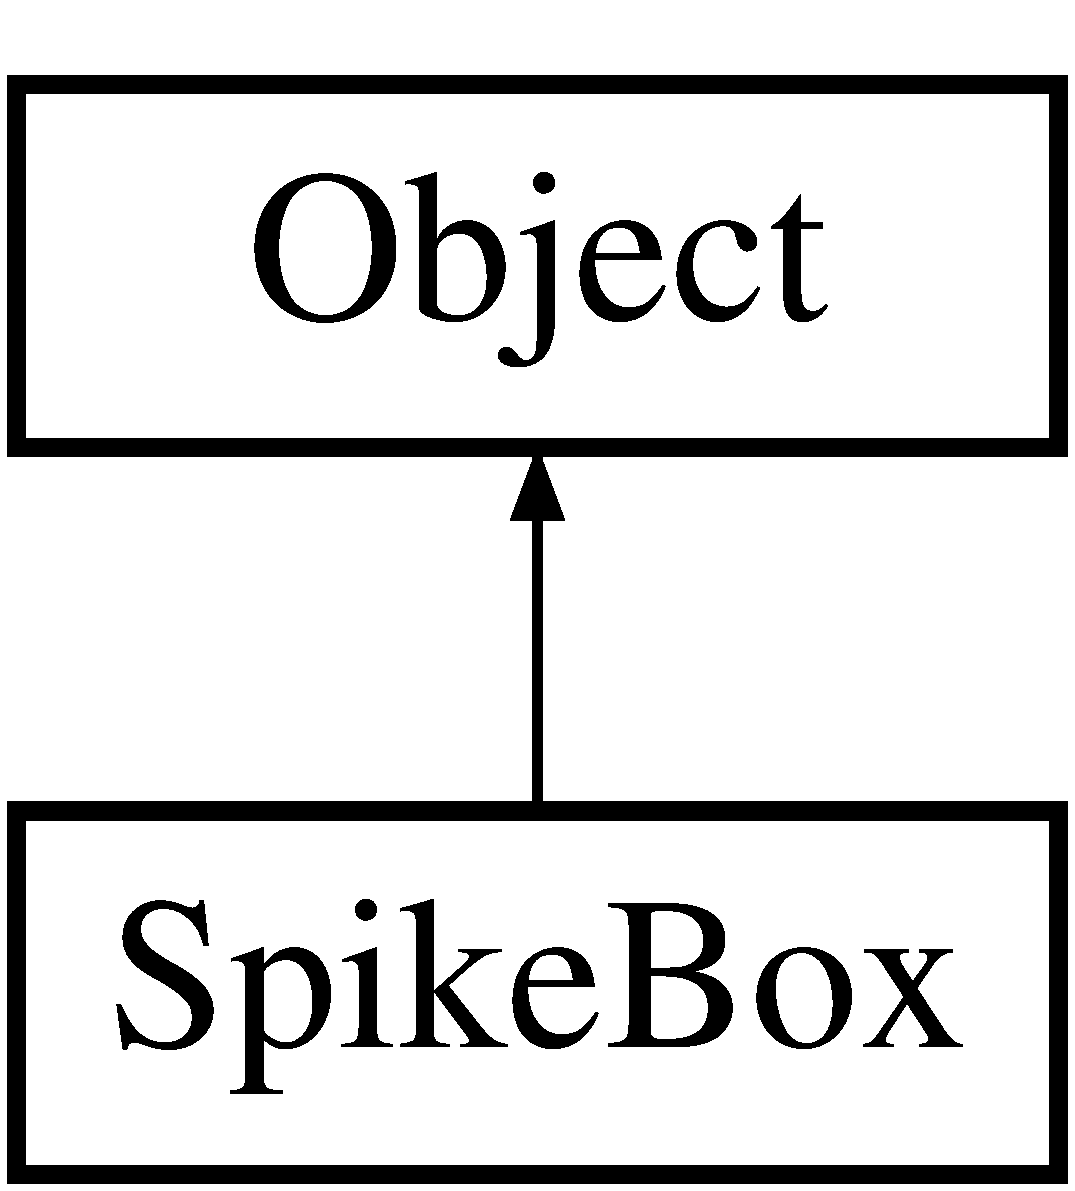
\includegraphics[height=2.000000cm]{class_spike_box}
\end{center}
\end{figure}
\subsection*{Public Member Functions}
\begin{DoxyCompactItemize}
\item 
\mbox{\Hypertarget{class_spike_box_a1bb832d0bb94295c3bb3e3276146820e}\label{class_spike_box_a1bb832d0bb94295c3bb3e3276146820e}} 
\hyperlink{class_spike_box_a1bb832d0bb94295c3bb3e3276146820e}{$\sim$\+Spike\+Box} ()
\begin{DoxyCompactList}\small\item\em Destructor. \end{DoxyCompactList}\item 
\mbox{\Hypertarget{class_spike_box_a7b3d5638f34943470a0045881ea78085}\label{class_spike_box_a7b3d5638f34943470a0045881ea78085}} 
\hyperlink{class_spike_box_a7b3d5638f34943470a0045881ea78085}{Spike\+Box} (\hyperlink{struct_vec2}{Vec2} position, \hyperlink{struct_vec2}{Vec2} scale, Body\+Type type, float32 density, float32 friction, char $\ast$texture, \hyperlink{struct_vec2}{Vec2} sprite\+Origin)
\begin{DoxyCompactList}\small\item\em Constructor. \end{DoxyCompactList}\item 
\mbox{\Hypertarget{class_spike_box_acff57f058cc8c29110fc52bc1ac66c0d}\label{class_spike_box_acff57f058cc8c29110fc52bc1ac66c0d}} 
virtual void \hyperlink{class_spike_box_acff57f058cc8c29110fc52bc1ac66c0d}{Init} () override
\begin{DoxyCompactList}\small\item\em Init. \end{DoxyCompactList}\item 
\mbox{\Hypertarget{class_spike_box_a76956f8a2c3071869c851f77b396aa38}\label{class_spike_box_a76956f8a2c3071869c851f77b396aa38}} 
virtual void \hyperlink{class_spike_box_a76956f8a2c3071869c851f77b396aa38}{Input} () override
\begin{DoxyCompactList}\small\item\em Input. \end{DoxyCompactList}\item 
\mbox{\Hypertarget{class_spike_box_a546f46c449d79576a6dd364dd28f08e6}\label{class_spike_box_a546f46c449d79576a6dd364dd28f08e6}} 
virtual void \hyperlink{class_spike_box_a546f46c449d79576a6dd364dd28f08e6}{Update} () override
\begin{DoxyCompactList}\small\item\em Update. \end{DoxyCompactList}\item 
\mbox{\Hypertarget{class_spike_box_a367ab98224d87535dcd037ee46de2231}\label{class_spike_box_a367ab98224d87535dcd037ee46de2231}} 
virtual void \hyperlink{class_spike_box_a367ab98224d87535dcd037ee46de2231}{Reset} () override
\begin{DoxyCompactList}\small\item\em Reset. \end{DoxyCompactList}\item 
virtual void \hyperlink{class_spike_box_a538790d5fe1e7619d693659f1e14cc44}{Collision} (\hyperlink{class_object}{Object} $\ast$instigator) override
\item 
\mbox{\Hypertarget{class_spike_box_a55e11ae1fdb92e34e384dc4ee00cd805}\label{class_spike_box_a55e11ae1fdb92e34e384dc4ee00cd805}} 
virtual Define\+Type \hyperlink{class_spike_box_a55e11ae1fdb92e34e384dc4ee00cd805}{get\+Define\+Type} () override
\begin{DoxyCompactList}\small\item\em Type of object. \end{DoxyCompactList}\end{DoxyCompactItemize}
\subsection*{Private Attributes}
\begin{DoxyCompactItemize}
\item 
\mbox{\Hypertarget{class_spike_box_af38562c097cdb89864ceced7647dad89}\label{class_spike_box_af38562c097cdb89864ceced7647dad89}} 
int \hyperlink{class_spike_box_af38562c097cdb89864ceced7647dad89}{Change\+VelocityX}
\begin{DoxyCompactList}\small\item\em Velocity X. \end{DoxyCompactList}\end{DoxyCompactItemize}
\subsection*{Additional Inherited Members}


\subsection{Member Function Documentation}
\mbox{\Hypertarget{class_spike_box_a538790d5fe1e7619d693659f1e14cc44}\label{class_spike_box_a538790d5fe1e7619d693659f1e14cc44}} 
\index{Spike\+Box@{Spike\+Box}!Collision@{Collision}}
\index{Collision@{Collision}!Spike\+Box@{Spike\+Box}}
\subsubsection{\texorpdfstring{Collision()}{Collision()}}
{\footnotesize\ttfamily virtual void Spike\+Box\+::\+Collision (\begin{DoxyParamCaption}\item[{\hyperlink{class_object}{Object} $\ast$}]{instigator }\end{DoxyParamCaption})\hspace{0.3cm}{\ttfamily [override]}, {\ttfamily [virtual]}}

Collision with other objects 
\begin{DoxyParams}{Parameters}
{\em instigator} & Objects name to collide with. \\
\hline
\end{DoxyParams}


Reimplemented from \hyperlink{class_object_a0af60ea226dcb885e69483452d34a47a}{Object}.



The documentation for this class was generated from the following file\+:\begin{DoxyCompactItemize}
\item 
D\+:/\+Multiplayer/include/spikebox.\+h\end{DoxyCompactItemize}

\hypertarget{struct_spike_box_info}{}\section{Spike\+Box\+Info Struct Reference}
\label{struct_spike_box_info}\index{Spike\+Box\+Info@{Spike\+Box\+Info}}


{\ttfamily \#include $<$networkmanager.\+h$>$}

\subsection*{Public Attributes}
\begin{DoxyCompactItemize}
\item 
\mbox{\Hypertarget{struct_spike_box_info_a27fffbfeaf328251eca084c589dc49b9}\label{struct_spike_box_info_a27fffbfeaf328251eca084c589dc49b9}} 
float {\bfseries PosX}
\item 
\mbox{\Hypertarget{struct_spike_box_info_ae2ac8d64043b7da65ec441b5770919be}\label{struct_spike_box_info_ae2ac8d64043b7da65ec441b5770919be}} 
float {\bfseries PosY}
\item 
\mbox{\Hypertarget{struct_spike_box_info_ae9ac2a746c9d5f5b080aad93ac93738a}\label{struct_spike_box_info_ae9ac2a746c9d5f5b080aad93ac93738a}} 
float {\bfseries Rotation}
\end{DoxyCompactItemize}


\subsection{Detailed Description}
Struct All the information that the spike box needs to receive and send 

The documentation for this struct was generated from the following file\+:\begin{DoxyCompactItemize}
\item 
D\+:/\+Multiplayer/include/networkmanager.\+h\end{DoxyCompactItemize}

\hypertarget{struct_vec2}{}\section{Vec2 Struct Reference}
\label{struct_vec2}\index{Vec2@{Vec2}}


{\ttfamily \#include $<$object.\+h$>$}

\subsection*{Public Member Functions}
\begin{DoxyCompactItemize}
\item 
\mbox{\Hypertarget{struct_vec2_a31ddae74bc80039c0a08f3e8a29fd924}\label{struct_vec2_a31ddae74bc80039c0a08f3e8a29fd924}} 
{\bfseries Vec2} (float32 x, float32 y)
\end{DoxyCompactItemize}
\subsection*{Public Attributes}
\begin{DoxyCompactItemize}
\item 
\mbox{\Hypertarget{struct_vec2_a186c8e91644c835bf422a09de2a7cedc}\label{struct_vec2_a186c8e91644c835bf422a09de2a7cedc}} 
float32 {\bfseries X}
\item 
\mbox{\Hypertarget{struct_vec2_adfc6433289a436891298d87144a0d02a}\label{struct_vec2_adfc6433289a436891298d87144a0d02a}} 
float32 {\bfseries Y}
\end{DoxyCompactItemize}


\subsection{Detailed Description}
Struct My vector 

The documentation for this struct was generated from the following file\+:\begin{DoxyCompactItemize}
\item 
D\+:/\+Multiplayer/include/object.\+h\end{DoxyCompactItemize}

\hypertarget{class_wall}{}\section{Wall Class Reference}
\label{class_wall}\index{Wall@{Wall}}
Inheritance diagram for Wall\+:\begin{figure}[H]
\begin{center}
\leavevmode
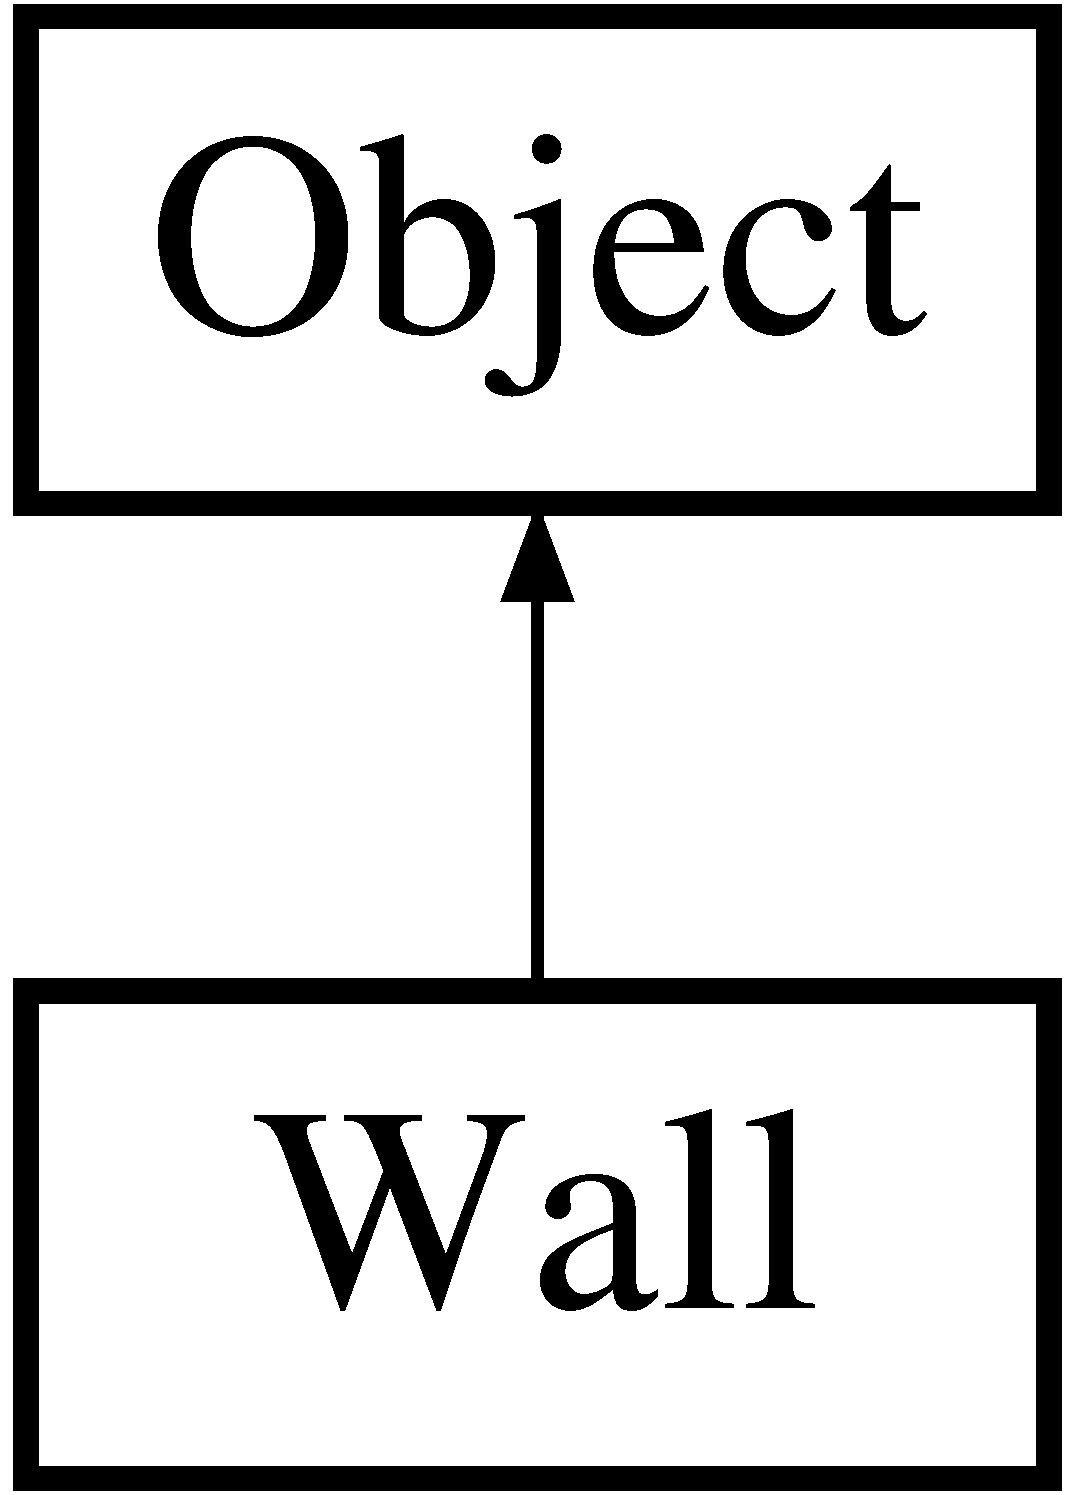
\includegraphics[height=2.000000cm]{class_wall}
\end{center}
\end{figure}
\subsection*{Public Member Functions}
\begin{DoxyCompactItemize}
\item 
\mbox{\Hypertarget{class_wall_a9a2992f2b533e1c160513d1e719f920c}\label{class_wall_a9a2992f2b533e1c160513d1e719f920c}} 
\hyperlink{class_wall_a9a2992f2b533e1c160513d1e719f920c}{$\sim$\+Wall} ()
\begin{DoxyCompactList}\small\item\em Destructor. \end{DoxyCompactList}\item 
\mbox{\Hypertarget{class_wall_a4bf1b54a7c78b0d8f474fd6bb5facbf5}\label{class_wall_a4bf1b54a7c78b0d8f474fd6bb5facbf5}} 
\hyperlink{class_wall_a4bf1b54a7c78b0d8f474fd6bb5facbf5}{Wall} (\hyperlink{struct_vec2}{Vec2} position, \hyperlink{struct_vec2}{Vec2} scale, Body\+Type type, float32 density, float32 friction, char $\ast$texture, \hyperlink{struct_vec2}{Vec2} sprite\+Origin)
\begin{DoxyCompactList}\small\item\em Constructor. \end{DoxyCompactList}\item 
\mbox{\Hypertarget{class_wall_a805d3f6cd3542b644c76cda032a7e167}\label{class_wall_a805d3f6cd3542b644c76cda032a7e167}} 
virtual void \hyperlink{class_wall_a805d3f6cd3542b644c76cda032a7e167}{Init} () override
\begin{DoxyCompactList}\small\item\em Init. \end{DoxyCompactList}\item 
\mbox{\Hypertarget{class_wall_a8e691c9f4d55ad0b2acce5a1faf1b4ae}\label{class_wall_a8e691c9f4d55ad0b2acce5a1faf1b4ae}} 
virtual void \hyperlink{class_wall_a8e691c9f4d55ad0b2acce5a1faf1b4ae}{Input} () override
\begin{DoxyCompactList}\small\item\em Input. \end{DoxyCompactList}\item 
\mbox{\Hypertarget{class_wall_aca64035887ce9058e8cc71be0042d564}\label{class_wall_aca64035887ce9058e8cc71be0042d564}} 
virtual void \hyperlink{class_wall_aca64035887ce9058e8cc71be0042d564}{Update} () override
\begin{DoxyCompactList}\small\item\em Update. \end{DoxyCompactList}\item 
virtual void \hyperlink{class_wall_a5a6c81f003e285ab96119d1aa983b82d}{Collision} (\hyperlink{class_object}{Object} $\ast$instigator) override
\item 
\mbox{\Hypertarget{class_wall_a6a1adf55f3ba0a2f0a878c03661eec0b}\label{class_wall_a6a1adf55f3ba0a2f0a878c03661eec0b}} 
virtual Define\+Type \hyperlink{class_wall_a6a1adf55f3ba0a2f0a878c03661eec0b}{get\+Define\+Type} () override
\begin{DoxyCompactList}\small\item\em Type of \hyperlink{class_object}{Object}. \end{DoxyCompactList}\end{DoxyCompactItemize}
\subsection*{Additional Inherited Members}


\subsection{Member Function Documentation}
\mbox{\Hypertarget{class_wall_a5a6c81f003e285ab96119d1aa983b82d}\label{class_wall_a5a6c81f003e285ab96119d1aa983b82d}} 
\index{Wall@{Wall}!Collision@{Collision}}
\index{Collision@{Collision}!Wall@{Wall}}
\subsubsection{\texorpdfstring{Collision()}{Collision()}}
{\footnotesize\ttfamily virtual void Wall\+::\+Collision (\begin{DoxyParamCaption}\item[{\hyperlink{class_object}{Object} $\ast$}]{instigator }\end{DoxyParamCaption})\hspace{0.3cm}{\ttfamily [inline]}, {\ttfamily [override]}, {\ttfamily [virtual]}}

Collision with other objects 
\begin{DoxyParams}{Parameters}
{\em instigator} & Objects name to collide with. \\
\hline
\end{DoxyParams}


Reimplemented from \hyperlink{class_object_a0af60ea226dcb885e69483452d34a47a}{Object}.



The documentation for this class was generated from the following file\+:\begin{DoxyCompactItemize}
\item 
D\+:/\+Multiplayer/include/wall.\+h\end{DoxyCompactItemize}

%--- End generated contents ---

% Index
\backmatter
\newpage
\phantomsection
\clearemptydoublepage
\addcontentsline{toc}{chapter}{Index}
\printindex

\end{document}
